\newpage
\section{PHƯƠNG TRÌNH QUY VỀ PHƯƠNG TRÌNH BẬC HAI}
\subsection{LÝ THUYẾT CẦN NHỚ}
\subsubsection{Phương trình dạng $\sqrt{ax^2+bx+c}=\sqrt{dx^2+ex+f}$}
Để giải phương trình $\sqrt{ax^2+bx+c}=\sqrt{dx^2+ex+f}$, ta thực hiện như sau:
\begin{itemize}
	\item Bình phương hai vế và giải phương trình nhận được;
	\item Thử lại các giá trị $x$ tìm được ở trên có thoả mãn phương trình đã cho hay không và kết luận nghiệm.
\end{itemize}
\subsubsection{Phương trình dạng $\sqrt{ax^2+bx+c}=dx+e$}
	Để giải phương trình $\sqrt{ax^2+bx+c}=dx+e$, ta thực hiện như sau:
\begin{itemize}
	\item Bình phương hai vế và giải phương trình nhận được;
	\item Thử lại các giá trị $x$ tìm được ở trên có thoả mãn phương trình đã cho hay không và kết luận nghiệm.
\end{itemize}
%-------------------------------------------------------------------------------------------------------------
\subsection{PHÂN LOẠI VÀ PHƯƠNG PHÁP GIẢI TOÁN}
\begin{dang}{Phương trình dạng $\sqrt{ax^2+bx+c}=\sqrt{dx^2+ex+f}$}
	Để giải phương trình $\sqrt{ax^2+bx+c}=\sqrt{dx^2+ex+f}$, ta thực hiện như sau:
	\begin{itemize}
		\item Bình phương hai vế và giải phương trình nhận được;
		\item Thử lại các giá trị $x$ tìm được ở trên có thoả mãn phương trình đã cho hay không và kết luận nghiệm.
	\end{itemize}
\end{dang}
\begin{vd}%[0D7H3-1]
	Giải phương trình $\sqrt{2x^2-4x-2}=\sqrt{x^2-x-2}$.
	\loigiai{
		Bình phương hai vế của phương trình, ta được
		$$2x^2-4x-2=x^2-x-2.$$
		Sau khi thu gọn ta được $x^2-3x=0$.\\ 
		Từ đó $x=0$ hoặc $x=3$.\\
		Thay lần lượt hai giá trị này của $x$ vào phương trình đã cho, ta thấy chỉ có $x=3$ thoả mãn.\\ 
		Vậy nghiệm của phương trình đã cho là $x=3$.
	}
\end{vd}

\begin{vd}%[0D7H3-1]
	Giải phương trình $\sqrt{2x^2-5x+2}-\sqrt{6-3x}=0$.
	\loigiai{
		\allowdisplaybreaks
		\begin{eqnarray*}
			\sqrt{2x^2-5x+2}-\sqrt{6-3x}=0 
			&\Rightarrow & \sqrt{2x^2-5x+2}=\sqrt{6-3x}\\
			&\Rightarrow &  2x^2-5x+2 = 6-3x\\
			& \Rightarrow &  x^2-x-2 = 0\\
			&\Rightarrow &  \hoac{& x = -1 \\ & x = 2.}
		\end{eqnarray*}
		Các nghiệm thỏa mãn phương trình ban đầu. \\ Vậy nghiệm của phương trình là $x=-1$ và $x=2$.
	}
\end{vd}

\begin{vd}%[0D7H3-1]
	Giải phương trình $\sqrt{x^2+3x}=2\sqrt{3x-2}$.
	\loigiai{
		\allowdisplaybreaks
		\begin{eqnarray*}
			\sqrt{x^2+3x}=2\sqrt{3x-2}
			&\Rightarrow &  x^2 + 3x = 4(3x - 2) \\
			&\Rightarrow & x^2 - 9x + 8 = 0\\
			&\Rightarrow & \hoac{& x = 1 \\ & x = 8.}
		\end{eqnarray*}
		Các nghiệm thỏa mãn phương trình ban đầu. \\ Vậy nghiệm của phương trình là $x=1$ và $x=8$.
	}
\end{vd}

\begin{dang}{Phương trình dạng $\sqrt{ax^2+bx+c}=dx+e$}
	Để giải phương trình $\sqrt{ax^2+bx+c}=dx+e$, ta thực hiện như sau:
	\begin{itemize}
		\item Bình phương hai vế và giải phương trình nhận được;
		\item Thử lại các giá trị $x$ tìm được ở trên có thoả mãn phương trình đã cho hay không và kết luận nghiệm.
	\end{itemize}	
\end{dang}
\begin{vd}%[0D7H3-2]
	Giải phương trình $\sqrt{2x^2-5x-9}=x-1$.
	\loigiai{
		Bình phương hai vế của phương trình ta được $$2x^2-5x-9=x^2-2x+1$$
		Sau khi thu gọn ta được $x^2-3x-10=0$.\\
		Từ đó $x=-2$ hoặc $x=5$.\\
		Thay lần lượt hai giá trị này của $x$ vào phương trình đã cho, ta thấy chỉ có $x=5$ thoả mãn.\\
		Vậy nghiệm của phương trình đã cho là $x=5$.
	}
	\begin{note}
		Với $x=-2$ thì vế phải âm, vế trái không âm. Do đó, ta có thể kết luận $x=-2$ không là nghiệm của phương trình đã cho mà không cần thử lại.
	\end{note}
\end{vd}
%VD2
\begin{vd}%[0D7H3-2]
	Giải phương trình $\sqrt{x^2-2x+5}=3x-1$.
	\loigiai{
		Bình phương hai vế của phương trình ta được $x^2-2x+5=9x^2-6x+1$.\\
		Sau khi thu gọn ta được $8x^2-4x-4=0$.\\
		Từ đó $x=1$ hoặc $x=-\dfrac{1}{2}$.\\
		Thay lần lượt hai giá trị này của $x$ vào phương trình đã cho, ta thấy chỉ có $x=1$ thoả mãn.\\
		Vậy nghiệm của phương trình đã cho là $x=1$.
	}
\end{vd}
%VD3
\begin{vd}%[0D7H3-2]
	Giải phương trình $\sqrt{2x^2+2}=x+1 $.
	\loigiai{
		Bình phương hai vế của phương trình ta được $2x^2+2=x^2+2x+1$.\\
		Sau khi thu gọn ta được $x^2-2x+1=0$.\\
		Từ đó $x=1$.\\
		Thay giá trị này của $x$ vào phương trình đã cho, ta thấy chỉ có $x=1$ thoả mãn.\\
		Vậy nghiệm của phương trình đã cho là $x=1$.
	}
\end{vd}
\begin{dang}{Bài toán thực tế}
	\begin{itemize}
		\item \textbf{Bước 1. Diễn tả mô hình bằng lời}\\
		Xác định đại lượng cần mô hình hóa và diễn tả bằng lời sự phụ thuộc của nó vào những đại lượng khác trong bài toán.
		\item \textbf{Bước 2. Chọn biến số}\\
		Xác định tất cả các đại lượng được dùng để diễn tả sự phụ thuộc bằng lời ở Bước 1. Dùng kí hiệu, chẳng hạn $ x $, để chỉ một đại lượng thích hợp nào đó và biểu diễn các đại lượng khác theo $ x $.
		\item \textbf{Bước 3. Thiết lập mô hình}\\
		Biểu diễn sự phụ thuộc ở Bước 1 như là một hàm số của biến số $ x $ đã được chọn ở Bước 2.
		\item \textbf{Bước 4. Sử dụng mô hình}\\
		Sử dụng hàm số đã thiết lập ở Bước 3 để trả lời các câu hỏi của bài toán.\\
		Kiểm tra sự phù hợp của mô hình.
	\end{itemize}
\end{dang}
\begin{vd}%[Dự án Bài Giảng 10-11 Nhóm Toán & LaTex, Nguyễn Anh Tuấn]%[0D7V3-6]
	Từ một tấm gỗ hình vuông cạnh $200$ cm. Cắt tấm gỗ đó tạo thành hình tam giác vuông, có tổng của một cạnh góc vuông và cạnh huyền bằng $120$ cm và cạnh góc vuông còn lại bằng $\dfrac{\sqrt3}{5}$ cạnh của tấm gỗ hình vuông. Hỏi cạnh huyền của tấm gỗ hình tam giác bằng bao nhiêu?
	\loigiai{
		Kí hiệu cạnh góc vuông $AB = x,\, 0 < x < 60$.\\ 
		Khi đó cạnh huyền $BC = 120 - x$.\\
		Cạnh góc vuông kia là $AC = \sqrt {BC^2 - AB^2} = \sqrt{120^2 - 240x} $.\\ 
		Theo giả thiết ta có 	
		$$	\sqrt{120^2 - 240x}=\dfrac{\sqrt3}{5}\cdot 200 \Leftrightarrow x=40.$$
		Vậy cạnh huyền  $BC = 80$.
	}
\end{vd}

\begin{vd}%[Dự án Bài Giảng 10-11 Nhóm Toán & LaTex, Nguyễn Anh Tuấn]%[0D7V3-6]
	\immini{Bác Việt sống và làm việc tại trạm hải đăng cách bờ biển $4$ km. Hằng tuần bác chèo thuyền vào vị trí gần nhất trên bờ biển là bến Bính để nhận hàng hoá do cơ quan cung cấp. Tuần này, do trục trặc về vận chuyển nên toàn bộ số hàng vẫn đang nằm ở thôn Hoành, bên bờ biển cách bến Bính $9{,}25$ km và sẽ được anh Nam vận chuyển trên con đường dọc bờ biển tới bến Bính bằng xe kéo. Bác Việt đã gọi điện thống nhất với anh Nam là họ sẽ gặp nhau ở vị trí nào đó giữa bến Bính và thôn Hoành để hai người có mặt tại đó cùng lúc, không mất thời gian chờ nhau. }{\begin{tikzpicture}[line cap=round, line join=round, font=\footnotesize, >=stealth, scale=0.5]
			\tikzset{label style/.style={font=\footnotesize}}
			\path (0,0) coordinate (B)
			(9.25,0) coordinate (C)
			(0,4) coordinate (A)
			(3,0) coordinate (M);
			\draw (M)--(A)--(B) node[midway, left]{$4$ km}--(C) (B)--(M) node[above, midway]{$x$ km};
			\draw[<->] ($(B)+(0,-0.5)$)--($(C)+(0,-0.5)$) node[below, midway]{$9,25$ km};
			\foreach\x/\y in {A/90,B/180,C/0,M/60} \draw[fill=black] (\x) circle (2pt) +(\y:0.6) node{$\x$};
			\draw pic[draw, angle radius=2mm]{right angle=A--B--M};
		\end{tikzpicture}	
	}Tìm vị trí hai người dự định gặp nhau, biết rằng vận tốc kéo xe của anh Nam là $5$ km/h và thuyền của bác Việt di chuyển với vận tốc $4$ km/h. Ngoài ra giả thiết rằng đường bờ biển từ thôn Hoành đến bến Bính là đường thẳng và bác Việt cũng luôn chèo thuyền tới một điểm trên bờ biển theo một đường thẳng.
	\loigiai{
		Trạm hải đăng ở vị tí $A$; bến Bính ở $B$ và thôn Hoành ở $C$. Giả sử bác Việt chèo thuyền cập bến ở vị trí $M$ và ta đặt $B M=x$ $(x>0)$. Để hai người không phải chờ nhau thì thời gian chèo thuyền bằng thời gian kéo xe nên ta có phương trình
		\begin{align*}
			&\frac{\sqrt{x^{2}+16}}{4}=\frac{9{,}25-x}{5} \Rightarrow 25\left(x^2+16\right)=16\left(x-9{,}25\right)^2\\
			\Rightarrow\ &9x^2+296x-969=0 \Rightarrow \hoac{&x=3\\ &x=-\frac{323}{9}.}
		\end{align*}
		Thử lại, kết hợp với điều kiện $x>0$, ta được $BM=x=3$ km.\\ Vậy vị trí gặp nhau cách thôn Bính $3$ km.
	}
\end{vd}
%-----------------------------------------------------------------------------
\subsection{BÀI TẬP RÈN LUYỆN}
\ind{PHẦN I.} \inden{Câu trắc nghiệm nhiều phương án lựa chọn. Mỗi câu hỏi học sinh chỉ chọn một phương án.}\\
\setcounter{ex}{0}
\Opensolutionfile{ans}[ans/1D7-Bai3-TN]%--Đặt tên 1D7-Bai3-Dang1-TN

\begin{ex}%[0D7N3-1]%[Dự án đề kiểm tra Toán 10 GKII NH23-24- Hoàng Vũ]%[THPT PHAN ĐÌNH PHÙNG -HN]
	[Trích đề GK2 - THPT Phan Đình Phùng - Tp. Hà Nội - Năm học 2023 - 2024]
	Bình phương cả hai vế của phương trình $\sqrt{x+2}=\sqrt{3x+1}$ rồi biến đổi, chuyển vế ta được phương trình nào sau đây?
	\choice
	{$2x+1=0$}
	{\True$2x-1=0$}
	{$3x-1=0$}
	{$2x+3=0$}
	\loigiai{
		$\sqrt{x+2}=\sqrt{3x+1}\Rightarrow x+2=3x+1\Rightarrow2x-1=0$.
	}
\end{ex}
\begin{ex}%[0D7H3-1]%[Duan15-CKII-HN23-24-Trần Xuân Hòa]%[Chuyen Hùng Vương - Phú Thọ]
	[Trích đề HK2 - THPT Chuyên Hùng Vương - Phú Thọ - Năm học 2023 - 2024]
	Số nào dưới đây là nghiệm của phương trình $\sqrt{2 x^2+x+3}=\sqrt{x^2+2 x+5}$?
	\choice
	{\True $x=2$}
	{$x=-3$}
	{$x=-2$}
	{$x=1$}
	\loigiai{
		\begin{eqnarray*}
			&&\sqrt{2 x^2+x+3}=\sqrt{x^2+2 x+5}\\
			&\Rightarrow&2x^2+x+3=x^2+2x+5\\
			&\Rightarrow&x^2-x-2=0\\
			&\Rightarrow&\hoac{&x=-1\\&x=2.}
		\end{eqnarray*}
		Thay $x=2$ vào phương trình ban đầu, thỏa mãn.\\
		Vậy $x=2$ là nghiệm.
	}
\end{ex}

%C:\Users\hppp\Desktop\Toan\ChuyenDeGK-CK-cacTruong\2.DA-SAULUOI-2024\Sp đợt 15\Sp ─æo╠¢╠út 15\Main\data\10-CaNuoc\0-TL-TN-THPT-DangHuyTru-Hue-HKII-NH23-24.tex
\begin{ex}%[0D7H3-2]%[Dự án đề kiểm tra Toán Khối 10 CK2 NH23-24-Dot 15- Nguyễn Hoàng Việt]%[THPT Đặng Huy Trứ - Thừa Thiên Huế]
	[Trích đề HK2 - THPT Đặng Huy Trứ - Thừa Thiên Huế - Năm học 2023 - 2024]
	Tập nghiệm của phương trình $\sqrt{2 x^2-4 x+9}=x+3$ là
	\choice
	{$\{10\}$}
	{$\{0\}$}
	{\True $\{0 ; 10\}$}
	{$\varnothing$}
	\loigiai{
		Ta có $\sqrt{2 x^2-4 x+9}=x+3\Rightarrow 2x^2-4x+9=\left(x+3\right)^2\Leftrightarrow x^2-10x=0\Leftrightarrow\hoac{&x=0\\&x=10.}$\\
		Thử lại ta nhận được được $2$ nghiệm.
	}
\end{ex}

%C:\Users\hppp\Desktop\Toan\ChuyenDeGK-CK-cacTruong\2.DA-SAULUOI-2024\Sp đợt 15\Sp ─æo╠¢╠út 15\Main\data\10-CaNuoc\0-TL-TN-THPT-DangHuyTru-Hue-HKII-NH23-24.tex
\begin{ex}%[0D7H3-2]%[Dự án đề kiểm tra Toán Khối 10 CK2 NH23-24-Dot 15- Nguyễn Hoàng Việt]%[THPT Đặng Huy Trứ - Thừa Thiên Huế]
	[Trích đề HK2 - THPT Đặng Huy Trứ - Thừa Thiên Huế - Năm học 2023 - 2024]
	Phương trình $\sqrt{x-1}=x-3$ có một nghiệm nằm trong khoảng nào sau đây?
	\choice
	{$\left(0 ; 2\right)$}
	{$\left(1 ; 3\right)$}
	{\True $\left(4 ; 7\right)$}
	{$\left(5 ; 9\right)$}
	\loigiai{
		Ta có $\sqrt{x-1}=x-3\Rightarrow x-1=x^2-6x+9\Leftrightarrow x^2-7x+10=0\Leftrightarrow\hoac{&x=2\\&x=5.}$\\
		Thử $2$ nghiệm vào phương trình ta thấy $x=5$ thỏa mãn.
	}
\end{ex}

%C:\Users\hppp\Desktop\Toan\ChuyenDeGK-CK-cacTruong\2.DA-SAULUOI-2024\Sp đợt 15\Sp ─æo╠¢╠út 15\Main\data\10-CaNuoc\0-TL-TN-THPT-DangHuyTru-Hue-HKII-NH23-24.tex
\begin{ex}%[0D7H3-1]%[Dự án đề kiểm tra Toán Khối 10 CK2 NH23-24-Dot 15- Nguyễn Hoàng Việt]%[THPT Đặng Huy Trứ - Thừa Thiên Huế]
	[Trích đề HK2 - THPT Đặng Huy Trứ - Thừa Thiên Huế - Năm học 2023 - 2024]
	Tập nghiệm của phương trình $\sqrt{4 x^2+2 x-6}=\sqrt{x^2+3 x+4}$ là
	\choice
	{$S=\left\{-\dfrac{5}{3}\right\}$}
	{$S=\{2\}$}
	{$S=\varnothing$}
	{\True $S=\left\{-\dfrac{5}{3} ; 2\right\}$}
	\loigiai{Ta có
		\begin{eqnarray*}
			& &\sqrt{4 x^2+2 x-6}=\sqrt{x^2+3 x+4}\\
			& \Rightarrow &	4x^2+2 x-6=x^2+3 x+4\\
			&\Leftrightarrow & 3x^2-x-10=0\\
			&\Leftrightarrow  & \hoac{&x=2\\&x=-\dfrac{5}{3}.}
		\end{eqnarray*}
		
		Thử $2$ nghiệm vào phương trình ta thấy thỏa mãn.
	}
\end{ex}

%C:\Users\hppp\Desktop\Toan\ChuyenDeGK-CK-cacTruong\2.DA-SAULUOI-2024\Sp đợt 15\Sp ─æo╠¢╠út 15\Main\data\10-CaNuoc\0-TL-TN-THPT-ThieuHoa-ThanhHoa-HKII-NH23-24.tex
\begin{ex}%[0D7N3-2]%[Dự án đề kiểm tra Toán 11 GHKII NH23-24-Nguyen Tran Anh Tuan]%[THPT Thiệu Hóa - Thanh Hóa]
	[Trích đề HK2 - THPT Thiệu Hóa - Thanh Hóa - Năm học 2023 - 2024]
	Phương trình $\sqrt{x-1}=x-3$ có số nghiệm là
	\choice
	{vô số nghiệm}
	{$2$}
	{\True $1$}
	{$0$}
	\loigiai{
		Điều kiện $x-3 \ge 0$ hay  $x \ge 3$.
		Khi đó bình phương hai vế phương trình đã cho ta được
		\begin{eqnarray*}
			x-1&=&(x-3)^2 \\
			x^2-7 x+10&=&0
		\end{eqnarray*}
		Suy ra $\hoac{&x=2\\&x=5.}$\\
		Thử lại với điều kiện ta có $x=5$ thỏa mãn.\\
		Vậy phương trình có nghiệm duy nhất là $x=5$.
	}
\end{ex}
%C:\Users\hppp\Desktop\Toan\ChuyenDeGK-CK-cacTruong\2.DA-SAULUOI-2024\Sp đợt 14\Main\data\10-TpHCM\0-TN-THPT-VinhLocB-TpHCM-GKII-NH23-24.tex
\begin{ex}%[0D7H3-1]%[Dự án đề kiểm tra Toán khối 10 GKII NH23-24-Dot14-Đặng Thế Vĩnh Hiển]%[Trường THPT Vĩnh Lộc B-TPHCM]
	[Trích đề GHKII THPT Vĩnh Lộc B - Tp. Hồ Chí Minh - Năm học 2023-2024]
	Số nghiệm của phương trình $\sqrt{2 x^2-9 x+1}=\sqrt{-x^2+1}$ là
	\choice{\True $1$}
	{$2$}
	{$0$}
	{$3$}
	\loigiai{Ta có \begin{eqnarray*}
			\sqrt{2 x^2-9 x+1}=\sqrt{-x^2+1}\Rightarrow2 x^2-9 x+1=-x^2+1\Leftrightarrow3 x^2-9 x=0\Rightarrow\hoac{&x=3\\&x=0.}
		\end{eqnarray*}
		Thay $x=3$ vào phương trình ban đầu ta được $\sqrt{-8}=\sqrt{-8}$ (Loại).\\Thay $x=0$ vào phương trình ban đầu ta được $\sqrt{1}=\sqrt{1}$ (Nhận).\\
		Vậy phương trình ban đầu có một nghiệm là $x=0$.
	}
\end{ex}
\begin{ex}%[Huỳnh Đức Vũ, Dự án 7]%[0D7H3-1]%Câu 11
	[Trích đề GHKII THPT Phạm Văn Đồng - Tp. Quãng Ngãi - Năm học 2024-2025]
	Tổng các nghiệm của phương trình $\sqrt{x^2+2x-3}=\sqrt{15-5x}$ là
	\choice
	{$ S=7$}
	{\True $ S=-7$}
	{$ S=6$}
	{$ S=4$}
	\loigiai{
		\allowdisplaybreaks
		\begin{eqnarray*}
			\sqrt{x^2+2x-3}=\sqrt{15-5x}&\Leftrightarrow&\heva{
				& 15-5x\ge 0\\&{x^2}+2x-3=15-5x}\\ 
			&\Leftrightarrow&\heva{
				& x\le 3\\&{x^2}+7x-18=0}\\&\Leftrightarrow&\heva{
				& x\le 3\\&\hoac{& x=2\\& x=-9}}\\ 
			&\Leftrightarrow& \hoac{& x=2\\& x=-9.}
		\end{eqnarray*}
		Vậy $ S=2-9=-7$.}
\end{ex}
%C:\Users\hppp\Desktop\Toan\ChuyenDeGK-CK-cacTruong\2.DA-SAULUOI-2024\Sp đợt 15\Sp ─æo╠¢╠út 15\Main\data\10-TpHCM\0-TN-THPT-NguyenThaiBinh-HCM-HKII-NH23-24.tex
\begin{ex}%[0D7H3-2]%[HKII-NGUYỄN THÁI BÌNH 2324]%[TheHung Nguyen]
	[Trích đề HKII THPT Nguyễn Thái Bình - Tp. Hồ Chí Minh - Năm học 2023-2024]
		Tập nghiệm của phương trình $\sqrt{x^2-3x+1}=\sqrt{x-2}$ là 
		\choice
		{$S=\left\{3;1\right\}$}
		{\True $S=\left\{3\right\}$}
		{$S=\left\{1\right\}$}
		{$S=\left\{3;6\right\}$}
		\loigiai{ $\sqrt{x^2-3x+1}=\sqrt{x-2}$  \quad (*)\\
			Bình phương hai vế của phương trình ta được $x^2-3x+1=x-2$.\\
			Thu gọn ta được $x^2-4x+3=0$.\\
			Do đó $x=1 \ \text{hoặc} \ x=3$.\\
			Thay $x=1$, $x=3$ vào (*)  ta thấy  chỉ có $x=3$ thỏa mãn.\\
			Vậy phương trình đã cho có tập nghiệm $S=\left\{3\right\}$.
		}
\end{ex}

%C:\Users\hppp\Desktop\Toan\ChuyenDeGK-CK-cacTruong\2.DA-SAULUOI-2024\Sp đợt 15\Sp ─æo╠¢╠út 15\Main\data\10-TpHCM\0-TN-THPT-NguyenThaiBinh-HCM-HKII-NH23-24.tex
\begin{ex}%[0D7H3-1]%[HKII-NGUYỄN THÁI BÌNH 2324]%[TheHung Nguyen]
		[Trích đề HKII THPT Nguyễn Thái Bình - Tp. Hồ Chí Minh - Năm học 2023-2024]
	Phương trình $\sqrt{x^2-6x-4}=\sqrt{x-4}$ có tập nghiệm là
	\choice
	{$\{0\}$}
	{\True $\{7\}$}
	{$\{0; 7\}$}
	{$\{0;-7\}$}
	\loigiai{		
		Bình phương hai vế ta được
		$\sqrt{x^2-6x-4}=\sqrt{x-4}\Rightarrow x^2-6x-4=x-4\Leftrightarrow x^2-7x=0\Leftrightarrow \hoac{& x=0 \\ & x=7.}$\\
		Thử lại ta thấy $x=0$ (loại), $x=7$ thỏa mãn phương trình.\\
		Tập nghiệm của phương trình đã cho là $\{7\}$.
	}
\end{ex}
\begin{ex}%[0D7H3-1]%[Dự án đề KT GKII - HKII Khối 10-11-12 NH24-25-Trịnh Văn Cảnh]%[THPT Lương Thế Vinh - Hà Nội]
	[Trích đề GHKII THPT Lương Thế Vinh - Tp. Hà Nội - Năm học 2024-2025]
	Tập nghiệm của phương trình $\sqrt{x^2-2x}=\sqrt{6-3x}$ có bao nhiêu phần tử?
	\choice
	{$1$}
	{Vô số}
	{$0$}
	{\True $2$}
	\loigiai{Ta có \allowdisplaybreaks
		\begin{eqnarray*}
			& & \sqrt{x^2-2x}=\sqrt{6-3x}\\
			&\Rightarrow & x^2-2x=6-3x\\
			&\Rightarrow & x^2+x-6=0\\
			&\Rightarrow & \hoac{&x=2\\&x=-3.}
		\end{eqnarray*}
		Thay $x=2$ và $x=-3$ vào phương trình đã cho ta thấy đều thỏa mãn.\\
		Vậy tập nghiệm của phương trình đã cho có $2$ phần tử.
	}
\end{ex}

%C:\Users\hppp\Desktop\Toan\ChuyenDeGK-CK-cacTruong\1.SAULUOI2025\SpDuAn-A-Dot10\data\HKII\0-TN-DS-TLN-THPT-NgoQuyen-HCM-HKII-NH24-25.tex
\begin{ex}%[Dự án đề kiểm tra Toán 10 HKII NH24-25- Lien Nguyen]%[THPT-Ngô Quyền - Tp HCM]%[0D7H3-2]%
	[Trích đề GHKII THPT Ngô Quyền - Tp. Hồ Chí Minh - Năm học 2024-2025]
	Cho phương trình $\sqrt{2x^2 - 5x - 9} = x-1$. Mệnh đề nào dưới đây đúng?
	\choice
	{Phương trình đã cho có hai nghiệm phân biệt trái dấu}
	{Phương trình đã cho có hai nghiệm phân biệt $x_1, x_2$ thỏa mãn $x_1 + x_2 = 3$}
	{\True Phương trình đã cho có nghiệm duy nhất $x = 5$}
	{Phương trình đã cho vô nghiệm}
	\loigiai{
		Bình phương hai vế của phương trình $\sqrt{2x^2 - 5x - 9} = x - 1$ ta được:
		\begin{eqnarray*}
			2x^2 - 5x - 9 &=& (x - 1)^2\\
			2x^2 - 5x - 9 &=& x^2 - 2x + 1\\
			x^2 - 3x - 10 &=& 0.
		\end{eqnarray*}
		Phương trình $x^2 - 3x - 10 = 0$ có $2$ nghiệm phân biệt $x_1=5$ và $x_2=-2$.\\
		Lần lượt thay $x_1=5$ và $x_2=-2$ vào phương trình $\sqrt{2x^2 - 5x - 9} = x-1$, ta thấy chỉ có $x_1=5$ thỏa mãn.\\
		Vậy phương trình đã cho có nghiệm duy nhất là $x = 5$.
	}
\end{ex}

%C:\Users\hppp\Desktop\Toan\ChuyenDeGK-CK-cacTruong\1.SAULUOI2025\SpDuAn-A-Dot10\data\GHKII\0-TN-TL-THPT-PhanDinhPhung-HaNoi-GHKII-NH24-25.tex
\begin{ex}%[Dự án đề kiểm tra Toán 10 GKII NH24-25-Nguyễn Sĩ Đạt]%[THPT Phan Đình Phùng - Hà Nội]%[0D7N3-1]
	[Trích đề GHKII THPT Phan Đình Phùng - Tp. Hà Nội - Năm học 2024-2025]
	Bình phương cả hai vế của phương trình $\sqrt{x^2+x+2}=\sqrt{3x+1}$ rồi biến đổi, thu gọn ta được phương trình nào sau đây?
	\choice
	{$-x^2+2x+1=0$}
	{$x^2+x+1=0$}
	{\True $x^2-2x+1=0$}
	{$x^2-2x-1=0$}
	\loigiai{Bình phương cả hai vế của phương trình, ta được
		$x^2+x+2=3x+1\Rightarrow x^2-2x+1=0$.}
\end{ex}

%C:\Users\hppp\Desktop\Toan\ChuyenDeGK-CK-cacTruong\1.SAULUOI2025\SpDuAn-A-Dot10\data\GHKII\0-TN-TL-THPT-PhanDinhPhung-HaNoi-GHKII-NH24-25.tex
\begin{ex}%[Dự án đề kiểm tra Toán 10 GKII NH24-25-Nguyễn Sĩ Đạt]%[THPT Phan Đình Phùng - Hà Nội]%[0D7V3-3]
	[Trích đề GHKII THPT Phan Đình Phùng - Tp. Hà Nội - Năm học 2024-2025]
	Cho phương trình $\sqrt{2x+m}=x$. Biết rằng tập hợp tất cả giá trị của $m$ để phương trình có hai nghiệm phân biệt là nửa khoảng $(a; b]$. Khi đó, giá trị của $b-a$ bằng
	\choice
	{\True $1$}
	{$2$}
	{$3$}
	{$4$}
	\loigiai{
		Điều kiện: $x\ge 0$.\\
		Bình phương hai vế của phương trình, ta được
		$\sqrt{2 x+m}=x  \Rightarrow x^{2}-2 x-m=0$.\\
		Ta có $\Delta =4+4m$, phương trình có hai nghiệm phân biệt nên $\Delta >0\Rightarrow m>-1$.\\
		Hai nghiệm của phương trình là 	$ x_{1}=1-\sqrt{1+m} , x_{2}=1+\sqrt{1+m}$.\\
		Do hai nghiệm của phương trình không âm nên $1-\sqrt{1+m}\ge 0\Rightarrow 1+m \leq 1 \Rightarrow m \leq 0 $.\\
		Vậy $m\in(-1;0]$ thỏa yêu cầu bài toán. Hay $a=-1$, $b=0$, suy ra $b-a=1$.
	}
\end{ex}

%C:\Users\hppp\Desktop\Toan\ChuyenDeGK-CK-cacTruong\1.SAULUOI2025\SpDuAn-A-Dot9\data\GHKII\0-TN-DS-TLN-TL-THPT-C-HaiHau-NamDinh-GHKII-NH24-25.tex
\begin{ex}%[0D7H3-2]%[0D3H1-2]%[Dự án đề kiểm tra Toán khối 10 GHKII NH24-25-Dot 9- Sy Truong]%[THPT C Hai Hau-Nam Dinh]
	[Trích đề GHKII tỉnh Nam Định - Năm học 2024-2025]
	Phương trình $\sqrt{x-2}+4=x$ có tập nghiệm là
	\choice
	{$S=\{3\}$}
	{$S=\{3; 6\}$}
	{\True $S=\{6\}$}
	{$S=\varnothing$}
	\loigiai{
		Ta có 
		\begin{eqnarray*}
			&&\sqrt{x-2}+4=x\\
			&\Rightarrow&\sqrt{x-2}=x-4\\
			&\Rightarrow&x-2=(x-4)^2\\
			&\Rightarrow&x-2=x^2-8x+16\\
			&\Rightarrow&x^2-9x+18=0\\
			&&\hoac{& x=3 \\ & x=6.}
		\end{eqnarray*}\\
		Thử lại ta thấy $ x=6 $ là nghiệm của phương trình.\\
		Vậy $S=\{6\}$.
	}
\end{ex}

%C:\Users\hppp\Desktop\Toan\ChuyenDeGK-CK-cacTruong\1.SAULUOI2025\SpDuAn-A-Dot9\data\GHKII\0-TN-DS-TLN-TL-THPT-ChuyenLuongTheVinh-DongNai-GHKII-NH24-25.tex
\begin{ex}%[0D7H3-2]%[Đề toán 10 - GHKII - THPT Chuyên Lương Thế Vinh - Tỉnh Đồng Nai - NH 24-25]%[Hieu Hieu Minh Minh] 
	[Trích đề GHKII - THPT Chuyên Lương Thế Vinh - Tỉnh Đồng Nai - Năm học 2024 - 2025]
	Số nghiệm của phương trình $\sqrt{x^2 + 4x - 1} = x - 3$ là
	\choice
	{\True $0$}
	{Vô số}
	{$2$}
	{$1$}
	\loigiai{
		Ta có 
		\begin{eqnarray*}
			&&\sqrt{x^2 + 4x - 1} = x - 3\,\,(*)\\
			&\Rightarrow & x^2+4x-1=(x-3)^2\\
			&\Rightarrow & 10x=10 \\
			&\Rightarrow & x = 1. 
		\end{eqnarray*}
		Thay $x=1$ vào phương trình $(*)$, ta có $x = 1$ không thỏa mãn nên phương trình đã cho vô nghiệm.\\
		Suy ra số nghiệm của phương trình là $0$.
	}
\end{ex}

%C:\Users\hppp\Desktop\Toan\ChuyenDeGK-CK-cacTruong\1.SAULUOI2025\SpDuAn-A-Dot9\data\GHKII\0-TN-DS-TLN-TL-THPT-LeLoi-KonTum-GHKII-NH24-25.tex
\begin{ex}%[0D7H3-1]%[Dự án đề kiểm tra Toán 10 HKII NH25-25-Nguyễn Thanh Phong]%[KonTum]
	[Trích đề thi GHKII - THPT Lê Lợi - Kon Tum - Năm học 2024 - 2025]
	Phương trình $\sqrt{2x^2-4x-2} = \sqrt{x^2-x-2}$ có nghiệm là
	\choice
	{$x = 4$}
	{$x = -2$}
	{$x = 0$}
	{\True $x = 3$}
	\loigiai{
		\begin{eqnarray*}
			&\sqrt{2x^2-4x-2} &= \sqrt{x^2-x-2} \quad (*)\\
			\Rightarrow &2x^2-4x-2 &= x^2-x-2 \\
			\Rightarrow  &x^2-3x & = 0\\
			\Rightarrow  &\hoac{&x=3  \\ &x=0}.
		\end{eqnarray*}
		Thử lại ta thấy $x=3$ thoả phương trình $(*)$.\\
		Vậy phương trình có nghiệm là $x=3$.
	}
\end{ex}

%C:\Users\hppp\Desktop\Toan\ChuyenDeGK-CK-cacTruong\1.SAULUOI2025\SpDuAn-A-Dot9\data\GHKII\0-TN-DS-TLN-TL-THPT-LeLoi-KonTum-GHKII-NH24-25.tex
\begin{ex}%[0D7H3-2]%[Dự án đề kiểm tra Toán 10 HKII NH25-25-Nguyễn Thanh Phong]%[KonTum]
	[Trích đề thi GHKII - THPT Lê Lợi - Kon Tum - Năm học 2024 - 2025]
	Số nghiệm của phương trình $\sqrt{x^2-3x+2} = x-2$ là
	\choice
	{$3$}
	{$0$}
	{$2$}
	{\True $1$}
	\loigiai{
		\begin{eqnarray*}
			&\sqrt{x^2-3x+2} &= x-2 \quad (*)\\
			\Rightarrow &x^2-3x+2 &= (x-2)^2 \\
			\Rightarrow  &x^2-3x & = x^2-4x+4\\
			\Rightarrow  &x=2.
		\end{eqnarray*}
		Thử lại ta thấy $x=2$ thoả phương trình $(*)$.\\
		Vậy phương trình có nghiệm là $x=2$.
	}
\end{ex}

%C:\Users\hppp\Desktop\Toan\ChuyenDeGK-CK-cacTruong\1.SAULUOI2025\SpDuAn-A-Dot9\data\GHKII\0-TN-DS-TLN-TL-THPT-SamSon-ThanhHoa-GHKII-NH24-25.tex
\begin{ex}%[0D7H3-2]%[Dự án đề kiểm tra Toán khối 10 GHKII-NH24-25-Dot9-Khắc Thiên]%[THPT Sầm Sơn-Thanh Hoá]
	[Trích đề thi GHKII THPT Sầm Sơn - Thanh Hoá - Năm học 2024 - 2025]
	Phương trình $\sqrt{x-1}=x-3$ có tập nghiệm là
	\choice
	{\True $S=\left\lbrace 5\right\rbrace $}
	{$S=\left\lbrace 2; 5\right\rbrace $}
	{$S=\emptyset$}
	{$S=\left\lbrace 2\right\rbrace $}
	\loigiai{Ta có \begin{eqnarray*}
			&&\sqrt{x-1}=x-3\\
			&\Rightarrow&x-1=(x-3)^2\\
			&\Rightarrow&x-1=x^2-6x+9\\
			&\Rightarrow&x^2-7x+10=0\\
			&\Rightarrow&\hoac{&x=5\\&x=2.}
		\end{eqnarray*}
		Thử lại ta thấy $x=5$ thoả mãn.\\
		Vậy tập nghiệm của phương trình đã cho là $S=\left\lbrace 5 \right\rbrace$.
	}
\end{ex}

%C:\Users\hppp\Desktop\Toan\ChuyenDeGK-CK-cacTruong\1.SAULUOI2025\SpDuAn-A-Dot9\data\GHKII\0-TN-DS-THPT-ChuyenNguyenDinhChieu-DongThap-GHKII-NH24-25.tex
\begin{ex}%[0D7H3-2]%[Dự án đề kiểm tra Toán 10 GHKII NH24-25-Thầy Hóa]%[THPT Chuyên Nguyễn Đình Chiều-Đồng Tháp]
	[Trích đề thi GHKII - THPT Chuyên Nguyễn Đình Chiều - Đồng Tháp - Năm học 2024 - 2025]
	Cho phương trình $\sqrt{x^2-2x+4}=2$. Chọn khẳng định đúng.
	\choice
	{Phương trình đã cho vô nghiệm}
	{Phương trình đã cho có đúng một nghiệm}
	{\True Tích các nghiệm của phương trình đã cho bằng $0$}
	{Tổng các nghiệm của phương trình đã cho bằng $-2$}
	\loigiai{
		Ta có $\begin{aligned}[t]
			&\sqrt{x^2-2x+4}=2\\
			&x^2-2x+4=4\\
			&x^2-2x=0\\
			&x=0\ \text{hoặc}\ x=2.
		\end{aligned}$\\
		Thử lại ta thấy $x\in\{0;2\}$ đều thỏa mãn.\\
		Vậy tích các nghiệm của phương trình đã cho bằng $0$.
	}
\end{ex}


\Closesolutionfile{ans}

\ind{PHẦN II.} \inden{Câu trắc nghiệm đúng sai. Trong mỗi ý a), b), c), d) ở mỗi câu, học sinh chọn đúng hoặc sai.}\\
\setcounter{ex}{0}
\begin{ex}%[0D7H3-3]%[GHKII - THPT Chuyên Nguyễn Đình Chiều - Đồng Tháp - Năm học 2024 - 2025]%[Trần Tiến Đức]
	[Trích đề thi GHKII - THPT Chuyên Nguyễn Đình Chiểu - Đồng Tháp - Năm học 2024 - 2025]
	Cho phương trình $\sqrt{2x^2-4x-5}=x$ (*). 
	\choiceTF
	{Bình phương hai vế của phương trình (*), ta được $x^2-4x+5=0$}
	{$x=-1$ là nghiệm của phương trình (*)}
	{\True Phương trình (*) có $1$ nghiệm}
	{\True Nghiệm của phương trình (*) cũng là nghiệm của phương trình $x-5=0$}
	\loigiai{
		Điều kiện của phương trình (*): $\heva{&2x^2-4x-5 \ge 0 \\ &x \ge 0.}$\\
		Bình phương hai vế (*), ta được $2x^2-4x-5 = x^2 \Leftrightarrow x^2-4x-5=0$.\\
		Phương trình $x^2-4x-5=0$ có hai nghiệm $x=-1$ (loại) và $x=5$ (nhận).\\
		Vậy phương trình (*) có nghiệm duy nhất $x=5$.
		\begin{itemchoice}
			\itemch Bình phương hai vế ta được $x^2-4x-5=0$.
			\itemch  $x=-1$ không thỏa mãn điều kiện $x \ge 0$.
			\itemch Phương trình (*) chỉ có một nghiệm là $x=5$.
			\itemch Nghiệm của (*) là $x=5$, cũng là nghiệm của $x-5=0$.
		\end{itemchoice}
	}
\end{ex}

\begin{ex}%[0D7H3-2]
	[Trích đề HKII - THPT Phú Nhuận - Tp. Hồ Chí Minh - Năm học 2024 - 2025]
	Cho phương trình $\sqrt{3x^2-9x+1}=2-x. \quad (1)$
	\choiceTF
	{Tổng các nghiệm của phương trình $(1)$ bằng $\dfrac{5}{2}$}
	{\True $x=-\dfrac{1}{2}$ là nghiệm của phương trình $(1)$}
	{\True Bình phương hai vế phương trình $(1)$ và thu gọn ta được $2x^2-5x-3=0$}
	{Phương trình $(1)$ có $2$ nghiệm phân biệt}
	\loigiai{ 
		Giải phương trình $\sqrt{3x^2-9x+1}=2-x \quad (1)$.\\
		Bình phương hai vế phương trình $(1)$, ta được 
		\[3x^2-9x+1=(2-x)^2 \Leftrightarrow 2x^2-5x-3=0 \Leftrightarrow \hoac{&x=3\\&x=-\dfrac{1}{2}.}\]
		Thử lại, ta được $x=-\dfrac{1}{2}$ là nghiệm của phương trình $(1)$.
		\begin{itemchoice}
			\itemch Tổng các nghiệm của phương trình $(1)$ bằng $-\dfrac{1}{2}$.
			\itemch Ta có $x=-\dfrac{1}{2}$ là nghiệm của phương trình $(1)$.
			\itemch Bình phương hai vế phương trình $(1)$, ta được $2x^2-5x-3=0$.
			\itemch Phương trình $(1)$ có một nghiệm duy nhất.
		\end{itemchoice}
	}	
\end{ex}

\begin{ex}%[0D7V3-1]
	[Trích đề HKII - THPT Trần Phú - Tp. Hồ Chí Minh - Năm học 2024 - 2025]
	Cho hàm số $y = f(x) = x^2 + mx - 2m - 3$, với $m$ là tham số thực.
	\choiceTF
	{\True $f(x)$ là tam thức bậc hai}
	{$f(2) < 0$ với mọi $m \in \mathbb{R}$}
	{\True Khi $m=1$, phương trình $\sqrt{f(x)} = \sqrt{x - 1}$ có đúng một nghiệm}
	{Có $5$ giá trị nguyên âm của tham số $m$ để hàm số $y = \dfrac{3}{\sqrt{f(x)}}$ luôn xác định với mọi $x \in \mathbb{R}$}
	\loigiai{
		\begin{itemchoice}
			\itemch Hàm số $f(x) = x^2 + mx - 2m - 3$, có hệ số $a = 1 \ne 0$ nên $f(x)$ là tam thức bậc hai.
			\itemch Ta có $f(2) = 4 + 2m - 2m - 3 = 1$, với mọi $m \in \mathbb{R}$. Do đó $f(2) > 0$, với mọi $m \in \mathbb{R}$.
			\itemch Với $m=1$, ta có $f(x) = x^2 + x - 5$.\\
			Xét phương trình $\sqrt{x^2 + x - 5} = \sqrt{x - 1}$.\qquad $(1)$\\
			Bình phương hai vế phương trình $(1)$ và thu gọn, ta được phương trình $x^2 = 4$.\\ Phương trình này có hai nghiệm phân biệt $x=2$ và $x=-2$.\\
			Thử lại, ta thấy chỉ có $x = 2$ thỏa mãn phương trình $(1)$.\\
			Do đó, phương trình $(1)$ có đúng một nghiệm.
			\itemch Điều kiện để hàm số $y = \dfrac{3}{\sqrt{f(x)}}$ xác định với mọi $x \in \mathbb{R}$ là $f(x) > 0$, $ \forall x \in \mathbb{R}$.\\
			Tam thức $f(x)$ có hệ số $a =1 > 0$ nên $f(x) > 0$, $ \forall x\in \mathbb{R}$ khi và chỉ khi 
			$$\Delta < 0 \Leftrightarrow m^2 + 4(2m + 3)<0 \Leftrightarrow m^2 + 8m + 12 < 0 \Leftrightarrow -6 < m < -2.$$
			Vậy có $3$ giá trị nguyên âm của tham số $m$ thỏa mãn bài toán là $m \in \{-5;-4;-3\}$.
		\end{itemchoice}
	}
\end{ex}

\begin{ex}%[0D7H3-5]%[Đề toán 10 - GHKII - THPT Chuyên Lương Thế Vinh - Tỉnh Đồng Nai - NH 24-25]%[Hieu Hieu Minh Minh] 
	[Trích đề GHKII - THPT Chuyên Lương Thế Vinh - Tỉnh Đồng Nai - Năm học 2024 - 2025]
	\immini{Hai con tàu đang ở tại vị trí $A$ (tàu $X$) và $B$ (tàu $Y$) cách nhau $10$ km cùng di chuyển về bến đỗ ở điểm $C$. Biết rằng hai tàu di chuyển theo đường thẳng cùng tốc độ $30$ km/h và phương di chuyển của hai tàu vuông góc với nhau (tham khảo hình vẽ). Tàu di chuyển từ $A$ đến $C$ trước tàu di chuyển từ $B$ trước 4 phút. Đặt $AC = x$ (km).
	\choiceTF
	{\True Thời gian tàu $X$ đi từ $A$ đến $C$ bằng $\dfrac{x}{30}$ giờ}
	{$\dfrac{BC}{30} - \dfrac{x}{30} = 4$}
	{$BC = \sqrt{x^2 - 100}$}
	{\True Khoảng cách giữa $A$ và $C$ là $6$ km}}{
		\begin{tikzpicture}[line join = round, line cap = round, scale=.8] 
			\coordinate[label = left:$C$] (C) at (0,0); 
			\coordinate[label = right:$B$] (B) at ($(C)+(2,0)$); 
			\coordinate[label = above:$A$] (A) at ($(C)+(0,3)$); 
			\draw[fill = gray!50] ($(C)!5pt!(B)$)--($(C)!5pt!(B)+(C)!5pt!(A)-(C)$)--($(C)!5pt!(A)$)--(C)--cycle;
			\draw (C)--(B)--(A)--cycle; 
			\foreach \x in {C,B,A} \fill[black] (\x) circle (1.5pt); 
		\end{tikzpicture} 
	}
	
	\loigiai{
		Ta có $4$ phút $= \dfrac{4}{60}$ giờ $= \dfrac{1}{15}$ giờ.\\
		\begin{itemchoice}
			
			\itemch
			Thời gian tàu $X$ đi từ $A$ đến $C$ là $\dfrac{x}{30}$ giờ.
			\itemch
			Thời gian tàu $Y$ đi từ $B$ đến $C$ là $\dfrac{BC}{30}$ giờ.\\
			Vì tàu $X$ đến $C$ trước tàu $Y$ $4$ phút nên $\dfrac{BC}{30} - \dfrac{x}{30} = \dfrac{1}{15}$ (*).
			\itemch 
			Áp dụng định lý Pythagore trong tam giác $ABC$ vuông tại $C$ \\
			$$AB^2 = AC^2 + BC^2 \Rightarrow 10^2 = x^2 + BC^2 \Rightarrow 100 = x^2 + BC^2 \text{  (**)}$$
			Suy ra $BC = \sqrt{100 -x^2}$.
			\itemch 
			Từ bước (*), ta có $BC = x + 2$.\\
			Thay $BC = x + 2$ vào phương trình (**), ta được $100 = x^2 + (x+2)^2$.\\
			Giải phương trình
			\begin{eqnarray*}
				&& 100 = x^2 + x^2 + 4x + 4 \\
				&\Leftrightarrow& 2x^2 + 4x - 96 = 0 \\
				&\Leftrightarrow& x^2 + 2x - 48 = 0\\
				&\Leftrightarrow& \hoac{&x = 6\\&x = -8.}
			\end{eqnarray*} 
			Vì $x$ phải dương nên $x = 6$.\\
			Do đó khoảng cách từ $A$ đến $C$ là $6$ km.
		\end{itemchoice}
	}
\end{ex}

\begin{ex}%[0D7H3-6]
	[Trích đề GHKII - THPT Marie Curie - Tp. Hồ Chí Minh - Năm học 2024 - 2025]
	\immini[thm]
	{Một con tàu biển $M$ rời cảng $O$ và chuyển động thẳng theo phương tạo với bờ biển một góc $60^\circ$. Trên bờ biển có hai đài quan sát $A$ và $B$ nằm về hai phía so với cảng $O$ và lần lượt cách cảng $O$ khoảng cách $1$ km và $3$ km (như hình vẽ). Đặt độ dài của $MO$ là $x$ (km).
		\choiceTF
	{$MB^2 = MO^2 + OB^2 + 2MO\cdot OB\cdot \cos{\widehat{MOB}}$}
	{\True Biểu diễn khoảng cách từ tàu đến $B$ theo $x$, ta được $MB = \sqrt{x^2 -3x + 9}$}
	{Biểu diễn khoảng cách từ tàu đến $A$ theo $x$, ta được $MA = \sqrt{x^2 - x + 1}$}
	{\True Để khoảng cách từ tàu đến $B$ bằng khoảng cách từ tàu đến $A$ thì $x = 2$ km}}
	{\begin{tikzpicture}
			\coordinate (O) at (0,0);
			\coordinate (A) at (-1.5,0);
			\coordinate (B) at (4.5,0);
			\coordinate (M) at ($(O)!1!60:(B)$);
			\draw (O)--(B)--(M)--(A) (A)--(O)--(M);
			\foreach \i in {O,A,B}
			\draw[fill=black] (\i) circle(1pt) node[below]{$\i$};
			\draw (M) circle (1pt)node[above]{$M$};
			\draw ($(O)!0.5!(B)$)node[below]{$3$ km};
			\draw ($(O)!0.5!(M)$)node[right]{$x$ km};
			\draw ($(O)!0.5!(A)$)node[below]{$1$ km};
			\draw pic[draw, angle radius=4mm]{angle=B--O--M}
			pic[" $60^\circ$",angle radius=13mm]{angle=B--O--M};
	\end{tikzpicture}}

	\loigiai{
		\begin{itemchoice}
			\itemch Áp dụng định lý cosin trong tam giác $OMB$, ta được $MB^2 = MO^2 + OB^2 - 2MO\cdot OB\cdot \cos{\widehat{MOB}}$.
			\itemch Ta có $MB^2 = MO^2 + OB^2 - 2MO\cdot OB\cdot \cos{\widehat{MOB}}=x^2+3^2-2\cdot x\cdot 3\cdot \cos 60^\circ\Rightarrow MB=\sqrt{x^2-3x+9}$.
			\itemch Áp dụng định lý cosin trong tam giác $OMA$, ta được $$MA^2=OM^2+OA^2-2\cdot OM\cdot OA\cdot \cos \widehat{OMA}=x^2+1^2-2\cdot x\cdot 1\cdot \cos 120^\circ\Rightarrow MA=\sqrt{x^2+x+1}.$$
			\itemch Khoảng cách từ tàu đến $B$ bằng khoảng cách từ tàu đến $A$ thì 
			\begin{eqnarray*}
				&&MB=MA\\
				&\Leftrightarrow& \sqrt{x^2-3x+9}=\sqrt{x^2+x+1}\\
				&\Rightarrow& x^2-3x+9=x^2+x+1\\
				&\Rightarrow& 4x=8\\
				&\Rightarrow& x=2.
			\end{eqnarray*}
			Thử lại, ta được $x=2$ là nghiệm của phương trình.
		\end{itemchoice}
		
	}
\end{ex}
\Closesolutionfile{ans}


\ind{PHẦN III.} \inden{Câu trắc nghiệm trả lời ngắn. Học sinh trả lời các câu hỏi sau.}\\
\setcounter{ex}{0}
\Opensolutionfile{ans}[ans/1D7-Bai3-DS]%--Đặt tên 1D7-Bai3-DS
%C:\Users\hppp\Desktop\Toan\ChuyenDeGK-CK-cacTruong\1.SAULUOI2025\SpDuAn-A-Dot9\data\GHKII\0-TN-DS-TLN-TL-THPT-LeLoi-KonTum-GHKII-NH24-25.tex
\begin{ex}%[0D7H3-2]%[Dự án đề kiểm tra Toán 10 HKII NH25-25-LamNguyen]%[KonTum]
	[Trích đề thi GHKII - THPT Lê Lợi - Kon Tum - Năm học 2024 - 2025]
	Cho phương trình $\sqrt{2x^2+3x-4}=5x-6$. Tổng các nghiệm của phương trình bằng $\dfrac{a}{b}$ với $a,\,b \in \mathbb{N}^*$ và $\dfrac{a}{b}$ là phân số tối giản. Tính tổng $a+b$.
	\shortans[oly]{$63$}
	\loigiai{Bình phương hai vế phương trình, ta được:
		\allowdisplaybreaks
		\begin{eqnarray*}
			& & 2x^2+3x-4=(5x-6)^2\\
			&\Rightarrow & 23x^2-63x+40=0\\
			&\Rightarrow & \hoac{&x=1\\&x=\dfrac{40}{23}.}
		\end{eqnarray*}
		Thay lần lượt các giá trị trên vào phương trình đã cho, ta thấy chỉ có $x=\dfrac{40}{23}$ thỏa mãn.\\
		Vậy $a=40, \,b=23$ và $a+b=63$.}
\end{ex}

\begin{ex}%[0D7V3-6]%[Dự án đề kiểm tra Toán 10 GHKII NH24-25- Phạm Văn Long]%[THPT Chuyên Lương Thế Vinh-Đồng Nai]
	[Trích đề GHKII - THPT Chuyên Lương Thế Vinh - Tỉnh Đồng Nai - Năm học 2024 - 2025]
	Bạn An muốn trồng một vườn hoa trên một mảnh đất hình chữ nhật và làm hàng rào bao quanh. An chỉ có đủ vật liệu để làm $40$ m hàng rào, nhưng An muốn diện tích vườn hoa ít nhất $84$ m$^2$. Hỏi chiều rộng của mảnh vườn ít nhất bằng bao nhiêu mét?
	\shortans[oly]{6}
	\loigiai{
		Gọi $x$ (m) là chiều rộng của mảnh vườn ($0<x<20$).\\
		Suy ra chiều dài của mảnh vườn là $20-x$ (m).\\
		Diện tích vườn hoa là $x\cdot (20-x)$ (m$^2$).\\
		Khi đó ta có bất phương trình $$x\cdot (20-x)\ge 84\Leftrightarrow -x^2+20x-84\ge 0\Leftrightarrow 6\le x \le 14.$$
		Vậy chiều rộng của mảnh vườn ít nhất bằng $6$ m.
	}
\end{ex}

%C:\Users\hppp\Desktop\Toan\ChuyenDeGK-CK-cacTruong\1.SAULUOI2025\SpDuAn-A-Dot9\data\GHKII\0-TN-DS-TLN-TL-THPT-NguyenChiThanh-TayNinh-GHKII-NH24-25.tex
\begin{ex}%[Đề thi GK2 lớp 10 THPT Nguyễn Chí Thanh-Tây Ninh năm học 2024-2025]%[Nguyễn Tấn Linh]%[0D7V3-6]
	[Trích đề thi GK2 THPT Nguyễn Chí Thanh - Tây Ninh - Năm học 2024-2025]
	\immini[thm]
	{Một công ty muốn xây dựng hệ thống dây cáp từ trạm $A$ ở trên bờ biển đến một vị trí $B$ trên một hòn đảo. Hòn đảo cách bờ biển $6\,$km. Gọi $C$ là điểm trên bờ sao cho $BC$ vuông góc với bờ biển. Khoảng cách từ $A$ đến $C$ là $9\,$km. Người ta cần xác định một vị trí $D$ trên $AC$ để lắp đặt hệ thống dây theo đường gấp khúc $ADB$ có số tiền chi phí thấp nhất là $1170$ triệu đồng. Khi đó khoảng cách $CD$ bằng bao nhiêu km, biết rằng giá để lắp đặt mỗi km hệ thống dây trên bờ là $50$ triệu đồng và dưới nước là $130$ triệu đồng?\shortans[oly]{$2,5$}
	}
	{
		\begin{tikzpicture}[scale=0.6,line join=round,line cap=round,font=\footnotesize]
			\def\lengthCA{9}
			\def\lengthCB{6}
			\def\offset{0.5}
			\coordinate (C) at (0,0);
			\coordinate (A) at (\lengthCA, 0);
			\coordinate (B) at (0, \lengthCB);
			\coordinate (D) at (\lengthCA/2.25, 0);
			\coordinate (BV) at (-\offset, \lengthCB);
			\coordinate (CV) at (-\offset, 0);
			\coordinate (CH) at (0, -\offset);
			\coordinate (AH) at (\lengthCA, -\offset);
			\draw[dashed] (BV) -- (CV)
			(CH) -- (AH);
			\draw[thick] (B) -- (C) -- (A)
			(B) -- (D);
			\foreach \P in {A,B,C,D,BV,CV,CH,AH}
			\fill (\P) circle (3pt);
			\node[above right] at (A) {$A$};
			\node[above left] at (B) {$B$};
			\node[below left] at (C) {$C$};
			\node[above right] at (D) {$D$};
			\node[left] at ($(BV)!0.5!(CV)$) {6km};
			\node[below] at ($(CH)!0.5!(AH)$) {9km};
		\end{tikzpicture}
	}
	\loigiai{
		Gọi $CD=x$, (km, $0\leq x\leq 9$).\\
		Khi đó, $BD=\sqrt{BC^2+CD^2}=\sqrt{36+x^2}$, $DA=9-x$.\\
		Chi phí lắp đặt dây trên $BD$ là $130\sqrt{36+x^2}$ (triệu đồng).\\
		Chi phí lắp đặt dây trên $DA$ là $50(9-x)=450-50x$ (triệu đồng).\\
		Do đó, tổng chi phí lắp đặt là $130\sqrt{36+x^2}+450-50x$ (triệu đồng).\\
		Vì số tiền chi phí thấp nhất là $1170$ triệu đồng nên
		\begin{eqnarray*}
			130\sqrt{36+x^2} + 450 - 50x = 1170
			&\Leftrightarrow& 130\sqrt{36+x^2} = 720 + 50x \\
			&\Rightarrow& 16900(36+x^2) = (720+50x)^2 \\
			&\Leftrightarrow& 608400 + 16900x^2 = 518400 + 72000x + 2500x^2 \\
			&\Leftrightarrow& 14400x^2 - 72000x + 90000 = 0 \\
			&\Leftrightarrow& x = \dfrac{5}{2}.
		\end{eqnarray*}
		Thay $x=\dfrac{5}{2}$ vào phương trình $130\sqrt{36+x^2}+450-50x=1170$, ta nhận $x=\dfrac{5}{2}$.\\
		Vậy khoảng cách $CD=\dfrac{5}{2}=2,5$ km.
	}
\end{ex}

\begin{ex}%[0D7C3-6]%[Dự án đề kiểm tra Toán 10 GHKII NH23-24- Lê Minh Thiện Anh]%[THPT chuyên Hùng Vương- Phú Thọ]
	[Trích đề GK2 - THPT Chuyên Hùng Vương - Phú Thọ - Năm học 2023 - 2024]
	Một ngọn hải đăng đặt tại vị trí $A$ cách bờ biển một khoảng $AB=4$ km. Trên bờ biển có một cửa hàng lương thực đặt ở vị trí $C$ cách $B$ một khoảng $15$ km. Hàng tháng, để mua lương thực người canh hải đăng phải đi xuồng máy từ $A$ đến bến tàu $M$ (không trùng vị trí $B$) với vận tốc trung bình $10$ km/h rồi đi xe gắn máy đến $C$ với vận tốc trung bình $30$ km/h. Tính tổng quãng đường (theo đơn vị km) người đó phải đi, biết rằng thời gian đi từ $A$ đến $C$ là $54$ phút.
	\begin{center}
		\begin{tikzpicture}[font=\footnotesize, line join=round, line cap=round, >=stealth]
			\path 	(0,3) coordinate (A)
			(0,0) coordinate (B)
			(7,0) coordinate (C)
			(2.5,0) coordinate (M);
			\draw 	(M)--(A)--(B)--(C);
			\foreach \x /\goc in {A/90,B/-135,C/0,M/-90}
			\fill[black] (\x) circle (1pt)
			($(\x)+(\goc:3mm)$) node {$\x$};
		\end{tikzpicture}
	\end{center}
	\shortans[oly]{$17$}
	\loigiai{
		Đổi $54$ phút $=\dfrac{9}{10}$ giờ.\\
		Gọi khoảng cách từ vị trí $B$ đến $M$ là $x$ (km, $x>0$).\\
		Khi đó ta có $AB=4$ km, $BM=x$ km, $BC=15$ km, $MC=BC-BM=15-x$ (km).\\
		Tam giác $ABM$ vuông tại $B$, áp dụng định lý Pythagore ta có
		$$AM^2=AB^2+BM^2=4^2+x^2=16+x^2\Rightarrow AM=\sqrt{16+x^2}.$$
		Do đó khoảng cách từ vị trí $A$ đến $M$ là $\sqrt{16+x^2}$ km và vận tốc đi xuồng máy là $10$ km/h nên thời gian đi xuồng máy từ $A$ đến $M$ là $t_1=\dfrac{\sqrt{16+x^2}}{10}$ (giờ).\\	
		Khoảng cách từ $M$ đến $C$ là $15-x$ (km) và người đó đi xe gắn máy với vận tốc $30$ km/h nên thời gian đi xe gắn máy từ $M$ đến $C$ là $t_2=\dfrac{15-x}{30}$ (giờ).\\
		Thời gian người đó đi từ $A$ đến $C$ chính bằng tổng thời gian người đó đi từ $A$ đến $M$ và từ $M$ đến $C$ nên ta có $t_1+t_2=t=\dfrac{9}{10}$ (giờ).\\
		Khi đó ta có phương trình
		\begin{eqnarray*}
			& & \dfrac{\sqrt{16+x^2}}{10}+\dfrac{15-x}{30}=\dfrac{9}{10}\\
			&\Leftrightarrow & 3\sqrt{16+x^2}+15-x=27\\
			&\Leftrightarrow & 3\sqrt{16+x^2}=12+x.	\quad(1)
		\end{eqnarray*}	
		Bình phương cả hai vế của $(1)$ ta được 
		\begin{eqnarray*}
			& & 9\left(16+x^2\right)=(12+x)^2\\
			&\Leftrightarrow & 144+9x^2=144+24x+x^2\\
			&\Leftrightarrow & 8x^2-24x=0\\
			&\Leftrightarrow & x=3 \,\,(\text{do điều kiện } x>0).
		\end{eqnarray*}	
		Khoảng cách từ vị trí $B$ đến vị trí $M$ là $3$ km, khoảng cách từ vị trí $M$ đến vị trí $C$ là $12$ km, khoảng cách từ $A$ đến $M$ là $5$ km.\\
		Vậy tổng quãng đường người đó phải đi là $5+12=17$ km.
	}
\end{ex}

%C:\Users\hppp\Desktop\Toan\[1]DU-AN-SP\ToanVaLaTeX\HK2-2024-2025\10-11-EX-HK2-2425-Dot-1_TVN-121\Data\0-HK2-1-NguyenThuongHien-M25-2425.tex
\begin{ex}%[Dự án 10-11-12EX-HK2-2425]%[Đề thi HK2 Lớp 10 THPT Nguyễn Thượng Hiền]%[Anh Duy]%[0D7H3-1]
	[Trích đề HK2 - THPT Nguyễn Thượng Hiền - Tp. Hồ Chí Minh - Năm học 2024 - 2025]
	\immini[thm]{Cho hai hàm số $y = f(x)$ và $y = g(x)$ có đồ thị như hình vẽ. Khi đó, tổng các nghiệm của phương trình $\sqrt{f(x)} = \sqrt{g(x)}$ là bao nhiêu?}{	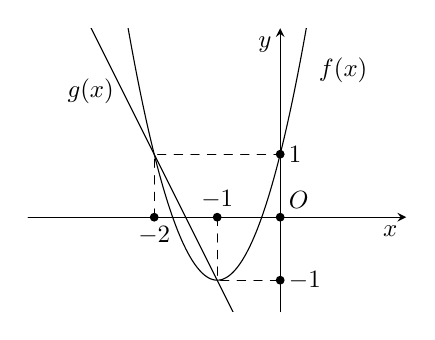
\begin{tikzpicture}[line join=round, line cap=round,>=stealth,scale=.8]
			\tikzset{every node/.style={scale=0.9}}
			\def\xmin{-4} \def\xmax{2}\def\ymin{-1.5}\def\ymax{3}
			\draw[->] (\xmin,0)--(\xmax,0) node[below left] {$x$};
			\draw[->] (0,\ymin)--(0,\ymax)  node[below left] {$y$};
			\clip (\xmin,\ymin) rectangle (\xmax,\ymax);
			\draw[dashed] (-1,0)|-(0,-1) (-2,0)|-(0,1);
			\fill (0,0)node[above right]{$O$} circle(2pt)
			(-2,0)node[below]{$-2$} circle(2pt)
			(-1,0)node[above]{$-1$} circle(2pt)
			(0,1)node[right]{$1$} circle(2pt)
			%	(-1,-1)node[above]{$1$} circle(2pt)
			(0,-1)node[right]{$-1$} circle(2pt)
			(1,2) node[above]{$f(x)$}
			(-2.5,2)node[left]{$g(x)$}
			;
			\begin{scope}
				\clip (\xmin,\ymin) rectangle (\xmax,\ymax);
				\draw[samples=200,domain=\xmin:\xmax,smooth,variable=\x] plot
				(\x,{2*(\x)^2+4*(\x)+1});
			\end{scope}
			\begin{scope}
				\clip (\xmin,\ymin) rectangle (\xmax,\ymax);
				\draw[samples=200,domain=\xmin:\xmax,smooth,variable=\x] plot
				(\x,{-2*(\x)-3});
			\end{scope}
	\end{tikzpicture}}
	\shortans[oly]{-2}
	\loigiai{
		Điều kiện $f(x)\ge 0$, $g(x)\ge 0$. Khi đó ta có $\sqrt{f(x)}=\sqrt{g(x)}\Rightarrow f(x)=g(x)$.\\
		Dựa vào đồ thị, đồ thị hai hàm số cắt nhau tại $(-2;1)$ và $(-1;-1)$.\\
		Mà $f(x)\ge 0$, $g(x)\ge 0$ nên phương trình có nghiệm $x=-2$.\\
		Vậy tổng các nghiệm của phương trình là $-2$.
	}
\end{ex}
\Closesolutionfile{ans}


\ind{PHẦN IV.} \inden{Tự luận.}\\
\setcounter{ex}{0}
\begin{bt}%[Vovanle]%[0D7H3-1]
	Giải các phương trình sau
	\begin{multicols}{2}
		\begin{enumerate}[1)]
			\item $\sqrt{2x^2-4x-2}=\sqrt{x^2-x-2}$.
			\item $\sqrt{3x^2-6x+1}=\sqrt{-2x^2-9x+1}$.
			\item $\sqrt{2x^2-3x-5}=\sqrt{x^2-7}$.
			\item $\sqrt{3x^2+6x+3}=\sqrt{2x^2-5x+3}$.
		\end{enumerate}
	\end{multicols}
	\loigiai{
		\begin{enumerate}[1)]
			\item $\sqrt{2x^2-4x-2}=\sqrt{x^2-x-2}$.\\
			Bình phương hai vế của phương trình ta được $2x^2-4x-2=x^2-x-2$.\\
			Sau khi thu gọn ta được $x^2-3x=0$.\\
			Từ đó tìm được $ x=0$ hoặc $x=3$.\\
			Thay lần lượt hai giá trị này vào phương trình đã cho, ta thấy chỉ có $x=3$ thỏa mãn.\\
			Vậy nghiệm của phương trình đã cho là $x=3$.
			\item $\sqrt{3x^2-6x+1}=\sqrt{-2x^2-9x+1}$.\\
			Bình phương hai vế của phương trình ta được $3x^2-6x+1=-2x^2-9x+1$.\\
			Sau khi thu gọn ta được $5x^2+3x=0$.\\
			Từ đó tìm được $ x=0$ hoặc $x=-\dfrac{3}{5}$.\\
			Thay lần lượt hai giá trị này vào phương trình đã cho, ta thấy $x=0$ và $x=-\dfrac{3}{5}$ thỏa mãn.\\
			Vậy tập nghiệm của phương trình đã cho là $S=\left\{0;-\dfrac{3}{5}\right\}$.
			\item $\sqrt{2x^2-3x-5}=\sqrt{x^2-7}$.\\
			Bình phương hai vế của phương trình ta được $2x^2-3x-5=x^2-7$.\\
			Sau khi thu gọn ta được $x^2-3x+2=0$.\\
			Từ đó tìm được $x=1$ hoặc $x=2$.\\
			Thay lần lượt giá trị này vào phương trình đã cho, ta thấy không có giá trị nào thỏa mãn.\\
			Vậy tập nghiệm của phương trình đã cho là $S=\varnothing$.
			\item Ta có
			\allowdisplaybreaks
			\begin{eqnarray*}
				&&\sqrt {3x^2+6x+3}=\sqrt {2x^2-5x+3}\\
				&\Leftrightarrow& \heva{& 3x^2+6x+3\geq 0\\& 2x^2-5x+3\geq 0\\& 3x^2+6x+3=2x^2-5x+3}\Leftrightarrow \heva{& \hoac{& x\leq 1\\& x\geq \dfrac{3}{2}}\\& x^2+11x=0 }\Leftrightarrow \heva{& \hoac{& x\leq 1\\ & x\geq \dfrac{3}{2}}\\& \hoac{& x=0\\& x=-11}}\Leftrightarrow \hoac{& x=0\\& x=-11.}
			\end{eqnarray*}
			Vậy phương trình có tập nghiệm $S=\{0;-11\}$.
		\end{enumerate}
	}
\end{bt}

\begin{bt}%[Vovanle]%[0D7H3-2]
	Giải các phương trình sau
	\begin{multicols}{2}
		\begin{enumerate}[1)]
			\item $\sqrt{2x^2-5x-9}=x-1$.
			\item $\sqrt{2x^2+x+13}=1-x$.
			\item $\sqrt{3x^2-13x+14}=x-3$.
			\item $\sqrt{-x^2+9x-5}=x$.
		\end{enumerate}
	\end{multicols}
	\loigiai{
		\begin{enumerate}[1)]
			\item $\sqrt{2x^2-5x-9}=x-1$.\\
			Bình phương hai vế của phương trình ta được $2x^2-5x-9=x^2-2x+1$.\\
			Sau khi thu gọn ta được $x^2-3x-10=0$.\\
			Từ đó tìm được $x=-2$ hoặc $x=5$.\\
			Thay lần lượt vào phương trình đã cho, ta thấy chỉ có $x=5$ thỏa mãn.\\
			Vậy nghiệm của phương trình đã cho là $x=5$.\\
			\item $\sqrt{2x^2+x+13}=1-x$.\\
			Bình phương hai vế của phương trình ta được $2x^2+x+3=1-2x+x^2$.\\
			Sau khi thu gọn ta được $x^2+3x+2=0$.\\
			Từ đó tìm được $x=-1$ hoặc $x=-2$.\\
			Thay lần lượt vào phương trình đã cho, ta thấy $x=-1$ hoặc $x=-2$ thỏa mãn.\\
			Vậy tập nghiệm của phương trình đã cho là $S=\{-1;-2\}$.
			\item $\sqrt{3x^2-13x+14}=x-3$.\\
			Bình phương hai vế của phương trình ta được $3x^2-13x+14=x^2-6x+9$.\\
			Sau khi thu gọn ta được $2x^2-7x+5=0$.\\
			Từ đó tìm được $ x=1$ hoặc $x=\dfrac{5}{2}$.\\
			Thay lần lượt vào phương trình đã cho, ta thấy không có giá trị nào thỏa mãn.\\
			Vậy tập nghiệm của phương trình đã cho là $S=\varnothing$.
			\item Ta có
			\begin{align*}
				\sqrt {-x^2+9x-5}=x &\Leftrightarrow \heva{& x\ge 0 \\ & -x^2+9x-5=x^2}\\
				&\Leftrightarrow \heva{& x\ge 0 \\ & 2x^2-9x+5=0 }\\
				&\Leftrightarrow x=\dfrac{9\pm \sqrt {41}}{4}.
			\end{align*}
			Vậy phương trình trên có $2$ nghiệm.
		\end{enumerate}
	}
\end{bt}

\begin{bt}%[Vovanle]%[0D7V3-4]
	Giải các phương trình sau
	\begin{multicols}{2}
		\begin{enumerate}[1)]
			\item $x^2-2x-8=4\sqrt{(4-x)(x+2)}$.
			\item $2\sqrt{x^2-8x}=x^2-8x-3$.
			\item $5\sqrt{x^3+x^2-2x}=2x^2+6x-2$.
			\item $13\sqrt{x^3+x^2-6x}=5x^2+21x-12$.
		\end{enumerate}
	\end{multicols}
	\loigiai{
		\begin{enumerate}[1)]
			\item $x^2-2x-8=4\sqrt{(4-x)(x+2)}$.\\
			Đặt $t=\sqrt {-x^2+2x+8}$ ($t\geq 0$), khi đó phương trình trở thành \[-{t^2}=4t\Leftrightarrow \hoac{& t=0 \\ & t=-4\text{ (loại)}.}\]
			Với $t=0\Rightarrow \sqrt{-x^2+2x+8}=0\Leftrightarrow \hoac{& x=4\\& x=-2.}$\\
			Vậy phương trình có hai nghiệm.
			\item $2\sqrt{x^2-8x}=x^2-8x-3$.\\
			Đặt $t=\sqrt {x^2-8x}$, $t\geq 0$. Phương trình trở thành
			$$2t={t^2}-3\Leftrightarrow {t^2}-2t-3=0\Leftrightarrow \hoac{& t=-1\text{ (loại)}\\ & t=3\text{ (nhận)}.}$$
			Với $ t=3\Leftrightarrow \sqrt {x^2-8x}=3\Leftrightarrow x^2-8x-9=0\Leftrightarrow \hoac{& x=9 \\ & x=-1.}$\\
			Vậy tổng các nghiệm của phương trình bằng $8$.
			\item $5\sqrt{x^3+x^2-2x}=2x^2+6x-2$.\\
			Điều kiện xác định của phương trình ${x^3}+x^2-2x\geq 0 \Leftrightarrow \hoac{& x\geq 1 \\ & -2\leq x\leq 0.}$\\
			Ta có
			\[5\sqrt {{x^3}+x^2-2x}=2x^2+6x-2 \Leftrightarrow 5\sqrt {(x-1)\left(x^2+2x\right)}=2\left(x^2+2x\right)+2(x-1).\,\,(*)\]
			Ta thấy với $x=1$ không phải là nghiệm của phương trình $(*)$.\\
			Với $x\neq 1$ ta có phương trình
			\allowdisplaybreaks
			\begin{eqnarray*}
				(*)& \Leftrightarrow& 2\left(\dfrac{x^2+2x}{x-1} \right)-5\sqrt {\dfrac{x^2+2x}{x-1}}+2=0\\
				&\Leftrightarrow& \hoac{& \sqrt {\dfrac{x^2+2x}{x-1}}=\dfrac{1}{2} \\ & \sqrt {\dfrac{x^2+2x}{x-1}}=2}\Leftrightarrow \hoac{& \dfrac{x^2+2x}{x-1}=\dfrac{1}{4} \\ & \dfrac{x^2+2x}{x-1}=4 }\Leftrightarrow\hoac{& 4x^2+7x+1=0 \\	& x^2-2x+4=0 }\Leftrightarrow \hoac{& x=\dfrac{-7+\sqrt {33}}{8} \\ & x=\dfrac{-7-\sqrt {33}}{8}.}
			\end{eqnarray*}
			So với điều kiện $\hoac{& x\geq 1\\ &-2\leq x\leq 0}$, ta có hai nghiệm $ x=\dfrac{-7\pm \sqrt {33}}{8}$ thỏa mãn.
			\item $13\sqrt{x^3+x^2-6x}=5x^2+21x-12$.\\
			Điều kiện xác định của phương trình ${x^3}+x^2-6x\geq 0\Leftrightarrow \hoac{& x\geq 2 \\ &-3\leq x\leq 0. }$\\
			Ta có
			\[13\sqrt {{x^3}+x^2-6x}=5x^2+21x-12\Leftrightarrow 13\sqrt{(x-2)\left(x^2+3x\right)}=5\left(x^2+3x\right)+6(x-2).\quad(*)\]
			Ta thấy với $x=2$ không phải là nghiệm của phương trình $(*)$.\\
			Với $x\neq 2$ ta có phương trình
			\allowdisplaybreaks
			\begin{eqnarray*}
				(*)&\Leftrightarrow& 5\dfrac{x^2+3x}{x-2}-13\sqrt {\dfrac{x^2+3x}{x-2}}+6=0\\
				&\Leftrightarrow& \hoac{& \sqrt {\dfrac{x^2+3x}{x-2}}=\dfrac{3}{5} \\ & \sqrt {\dfrac{x^2+3x}{x-2}}=2 }\Leftrightarrow \hoac{& \dfrac{x^2+3x}{x-2}=\dfrac{9}{25} \\ & \dfrac{x^2+3x}{x-2}=4}\Leftrightarrow \hoac{& 25x^2+66x+18=0 \\ & x^2-x+8=0 }\Leftrightarrow \hoac{& x=\dfrac{-33+3\sqrt {71}}{25} \\ & x=\dfrac{-33-3\sqrt {71}}{25}.}
			\end{eqnarray*}
			So với điều kiện $\hoac{& x\geq 2\\& -3\leq x\leq 0}$, ta có hai nghiệm $ x=\dfrac{-33\pm 3\sqrt{71}}{25}$ thỏa mãn.
		\end{enumerate}
	}
\end{bt}
\begin{bt}%[0D7V3-6]
	\immini{Một ngọn hải đăng đặt tại vị trí $A$ cách bờ biển một khoảng cách $AB=4$ km. Trên bờ biển có một cái kho ở vị trí $C$ cách $B$ một khoảng là $7$ km. Người canh hải đăng có thể chèo thuyền từ $A$ đến vị trí $M$ trên bờ biển với vận tốc $3$ km/h rồi đi bộ đến $C$ với vận tốc $5$ km/h như hình bên. Tính khoảng cách từ vị trí $B$ đến $M$, biết thời gian người đó đi từ $A$ đến $C$ là $148$ phút.}
	{\begin{tikzpicture}[scale=0.8, line join=round, line cap=round,>=stealth]
			\def\h{1}\def\a{3}\def\b{6}
			\path
			(0:0) coordinate (B)
			(90:\a) coordinate (A)
			(0:\b) coordinate (C)
			($(C)!0.7!(B)$) coordinate (M)
			;
			% sông
			\draw (A)--(B)node[midway,sloped,below]{$4$ km}--(C)
			(A)--(M)
			(B)--++(180:\h) (C)--++(0:\h)
			;
			\draw[dashed] (B)--++(-90:\h) (C)--++(-90:\h);
			\draw[<->] ([yshift=-5mm]B)--([yshift=-5mm]C)node[midway,sloped,below]{$7$ km};
			\foreach \p/\q in{A/90,B/150,C/90,M/50}\fill(\p)circle(1pt)+(\q:.5)node{$\p$};
	\end{tikzpicture}}
	\loigiai{
		Đặt $BM=x$ km ($0<x<7$), khi đó $CM=7-x$ và $AM=\sqrt{16+x^2}$.\\
		Ta có tổng thời gian đi từ $A$ đến $M$ và từ $M$ đến $C$ là $148$ phút nên ta có
		\allowdisplaybreaks 
		\begin{eqnarray*}
			&&\dfrac{AM}{3}+\dfrac{MC}{5}=\dfrac{148}{60}\\
			&\Leftrightarrow&\dfrac{\sqrt{16+x^2}}{3}+\dfrac{7-x}{5}=\dfrac{37}{15}\\
			&\Leftrightarrow& 5\sqrt{16+x^2}=3x+16\\
			&\Leftrightarrow& 25(16+x^2)=(3x+16)^2\\
			&\Leftrightarrow& 16x^2-96x+144=0\\
			&\Leftrightarrow& x^2-6x+9=0\\
			&\Leftrightarrow& x=3 \text{ (thỏa điều kiện)}.
		\end{eqnarray*}
		Vậy $BM=3$ km.
	}	
\end{bt}
\begin{bt}%[0D7H3-6]%[Dự án đề kiểm tra Toán 10 GHKII NH23-24- Đoàn Minh Tâm]%[THPT Nguyễn Tất Thành - TPHCM]
	\immini{
		Hai trạm quan sát $A$, $B$ trên bờ biển nhìn thấy tàu $M$ đang tiến về cảng $O$
		(như hình vẽ). Hãy tính tàu $M$ còn cách
		cảng $O$ bao nhiêu km nữa? Biết $4MA = 5MB$.
	}{
		\begin{tikzpicture}[line join = round, line cap = round,>=stealth,font=\footnotesize,scale=1.8]
			\coordinate (A) at (0,0);
			\coordinate (O) at (1,0);
			\coordinate (B) at (3,0);
			\coordinate (M) at ($(O)!0.8!60:(B)$);
			\draw (M)--(A)--(B)--cycle (M)--(O);
			\draw pic[draw,angle radius=3mm,angle eccentricity=2.5,"$60^\circ$"] {angle = B--O--M}; % Vẽ góc BAC với tên nhãn \beta
			\foreach \x/\y in {A/180, B/0, O/-90, M/90}{\fill (\x) circle(1pt) ($(\x)+(\y:0.2)$) node{$\x$};}
			\foreach \a in {0,0.25,0.5,0.75,1,1.25,1.5,1.75,2,2.25,2.5,2.75,3} {\draw[thin] (\a,0)--(\a-0.05,-0.15); }
			\draw (.6,.2) node{$1$ km} (2,.2) node{$2$ km} (1.6,0.6) node{$x$ km};
		\end{tikzpicture}
		
		;	}
	\loigiai{
		Điều kiện $x>0$.\\
		Do $\widehat{MOB}=60^\circ\Rightarrow \widehat{MOA}=120^\circ$.\\
		Xét $\triangle MOA$, theo định lý cosin, ta có
		$$MA=MO^2+OA^2-2\cdot MO \cdot OA\cdot \cos MOA=x^2+x+1\Rightarrow MA=\sqrt{x^2+x+1}.$$
		Xét $\triangle MOB$, theo định lý cosin, ta có
		$$MB=MO^2+OB^2-2\cdot MO \cdot OB \cdot \cos MOB=x^2-2x+4\Rightarrow MB=\sqrt{x^2-2x+4}.$$
		Vậy ta được $M A=\sqrt{x^2+x+1}$, $M B=\sqrt{x^2-2 x+4}$.\\
		Khi đó
		\begin{eqnarray*}
			&4 M A=5 M B &\Leftrightarrow 4\sqrt{x^2+x+1}=5\sqrt{x^2-2 x+4}\\
			&&\Leftrightarrow 9 x^2-66 x+84=0 \\
			&&\Leftrightarrow \hoac{&x=\dfrac{11-\sqrt{37}}{3} \approx 1{,}64\\ &x=\dfrac{11+\sqrt{37}}{3}\approx 5{,}69.}
		\end{eqnarray*}
		Vậy $M$ cách cảng $O$ khoảng $1{,}64$ km hay $5{,}69$ km.
	}
\end{bt}
\begin{bt}%[0D7V3-6]
	\immini{Một con tàu $M$ rời cảng $O$ và chuyển động theo phương tạo với bờ biển một góc $60^\circ $. Trên bờ biển có hai đài quan sát $A$ và $B$ nằm về hai phía so với cảng $O$ và lần lượt cách cảng $O$ khoảng cách $ 1 $ km và $ 2 $ km  (Hình bên).}{\begin{tikzpicture}[line join = round, line cap = round,>=stealth,font=\footnotesize,scale=1.8]
			\coordinate (A) at (0,0);
			\coordinate (O) at (1,0);
			\coordinate (B) at (3,0);
			\coordinate (M) at ($(O)!0.8!60:(B)$);
			\draw (M)--(A)--(B)--cycle (M)--(O);
			\draw pic[draw,angle radius=3mm,angle eccentricity=2.5,"$60^\circ$"] {angle = B--O--M}; % Vẽ góc BAC với tên nhãn \beta
			\foreach \x/\y in {A/180, B/0, O/-90, M/90}{\fill (\x) circle(1pt) ($(\x)+(\y:0.2)$) node{$\x$};}
			\foreach \a in {0,0.25,0.5,0.75,1,1.25,1.5,1.75,2,2.25,2.5,2.75,3} {\draw[thin] (\a,0)--(\a-0.05,-0.15); }
			\draw (.6,.2) node{$1$ km} (2,.2) node{$2$ km} (1.6,0.6) node{$x$ km};
	\end{tikzpicture}}
	\begin{enumEX}{1}
		\item Đặt độ dài của $MO$ là $x$ km. Biểu diễn khoảng cách từ tàu đến $A$ và từ tàu đến $B$ theo $x$.
		\item Tìm $x$ để khoảng cách từ tàu đến $B$ bằng $ \dfrac{4}{5} $ khoảng cách từ tàu đến $A$.
		\item Tìm $x$ để khoảng cách tử tàu đến $B$ nhỏ hơn khoảng cách từ tàu đến $O$ cảng 500 m. 
	\end{enumEX}
	\loigiai{
		\begin{enumEX}{1}
			\item Xét tam giác $MOB$ ta có:\\
			\begin{eqnarray*}
				{{MB}^{2}}&=&M{{O}^{2}}+O{{B}^{2}}-2OM\cdot OB\cdot\cos60{}^\circ\\
				{{MB}^{2}}&=&{{x}^{2}}+{{2}^{2}}-2\cdot x\cdot2\cdot\dfrac{1}{2}\\
				{{MB}^{2}}&=&{{x}^{2}}-2x+4\\
				MB&=&\sqrt{{{x}^{2}}-2x+4}.\\
			\end{eqnarray*}
			Xét tam giác $MOA$ ta có:
			\begin{eqnarray*}
				{{MA}^{2}}&=&M{{O}^{2}}+O{{A}^{2}}-2OM.OA.\cos\left( 180{}^\circ -60{}^\circ  \right)\\
				{{MA}^{2}}&=&{{x}^{2}}+{{1}^{2}}-2\cdot x\cdot 1\cdot\left( \dfrac{-1}{2} \right)\\
				{{MA}^{2}}&=&{{x}^{2}}+x+1\\
				MA&=&\sqrt{{{x}^{2}}+x+1}.\\
			\end{eqnarray*}
			\item Theo đề bài ta có:
			\begin{eqnarray*}
				&MB&=\dfrac{4}{5}MA\\
				\Leftrightarrow&\sqrt{{{x}^{2}}-2x+4}&=\dfrac{4}{5}\cdot\sqrt{{{x}^{2}}+x+1}\\
				\Rightarrow&{{x}^{2}}-2x+4&=\dfrac{16}{25}\cdot\left( {{x}^{2}}+x+1 \right) \\
				\Leftrightarrow&\dfrac{9}{25}{{x}^{2}}-\dfrac{66}{25}x+\dfrac{84}{25}&=0 \\
				\Rightarrow&\hoac{&x=\dfrac{11+\sqrt{37}}{3}\approx 5,7\\&x=\dfrac{11-\sqrt{37}}{3}\approx 1,64.}&\\
			\end{eqnarray*}
			
			Thay lần lượt các giá trị vào phương trình đã cho ta thấy $x=\dfrac{11+\sqrt{37}}{3}\approx 5,7$ và $x=\dfrac{11-\sqrt{37}}{3}\approx 1,64$ thỏa mãn.\\
			Vậy $x\approx 5,7$ hoặc $x\approx 1,64$ thỏa mãn đề bài.
			\item Theo đề bài ta có:\\
			\begin{eqnarray*}
				&OM&=MB+5\\
				\Leftrightarrow&x&=\sqrt{{{x}^{2}}-2x+4}+5\\
				\Leftrightarrow&x-5&=\sqrt{{{x}^{2}}-2x+4}\\
				\Rightarrow&{{x}^{2}}-10x+25&={{x}^{2}}-2x+4\\
				\Rightarrow&-8x&=-21 \\
				\Rightarrow&x&=\dfrac{21}{8}=2,625 \\
			\end{eqnarray*}
			Thử lại ta thấy $x=2,625$ thỏa mãn.
			Vậy $x=2,625$ thỏa mãn yêu cầu đề bài.
			
		\end{enumEX}
	}
\end{bt}
\begin{bt}%[0D7V3-6]
	Hằng ngày bạn Hùng đều đón bạn Minh đi học tại một vị trí trên lề đường thẳng đến trường. Minh đứng tại vị trí $A$ cách lề đường một khoảng $50 \mathrm{~m}$ để chờ Hùng. Khi nhìn thấy Hùng đạp xe đến địa điểm $B$, cách mình một đoạn $200 \mathrm{~m}$ thì Minh bắt đầu đi bộ ra lề đường để bắt kịp xe. Vận tốc đi bộ của Minh là $5 \mathrm{~km} / \mathrm{h}$, vận tốc xe đạp của Hùng là $15 \mathrm{~km} / \mathrm{h}$. Hãy xác định vị trí $C$ trên lề đường (hình bên dưới) để hai bạn gặp nhau mà không bạn nào phải chờ người kia (làm tròn kết quả đến hàng phần mười).
	\begin{center}
		\begin{tikzpicture}[thick,scale=1,nodes={scale=1}]
			\path 	(0:0) coordinate (A)
			++(90:1.7) coordinate (M)
			++(90:0.3) coordinate (H)
			++(180:0.3) coordinate (N)
			++(180:3) coordinate (C)
			++(180:4) coordinate (B);
			\path 	(N)
			++(-90:0.3) coordinate (P);	
			\draw (A)--(H)--(C)--(B)--cycle;
			\draw (A)--(C);
			\draw (M)--(H)--(N)--(P)--cycle;
			\foreach \x/ \goc in {A/0,B/-90,C/90,H/50} 
			\fill (\x) circle (1pt)
			($(\x)+(\goc:3mm)$) node {$\x$};
			\draw (B) node[above]{Hùng $\rightarrow$} (A) node[below left]{Minh};
			\draw (0,1) node[right] {$50$ m} (-3,0.8) node[below]{$200$ m};
			\draw[->] (135:1)--(140:1.5);
			
		\end{tikzpicture}
		
	\end{center}
	\loigiai{ Đặt $CH=x$, điều kiện $x>0$.\\
		Ta có $BC=\sqrt{BA^2-AH^2}-x=50\sqrt{15}-x.$\\
		$AC=\sqrt{HC^2+AH^2}=\sqrt{x^2+50^2}$.\\
		Thời gian của Hùng đi từ $B$ tới $C$ bằng $\dfrac{50\sqrt{15}-x}{15}$.\\
		Thời gian của Minh đi từ $A$ tới $C$ bằng $\dfrac{\sqrt{50^2+x^2}}{5}$.\\
		Hai bạn gặp nhau đúng thời điểm khi và chỉ khi $\dfrac{\sqrt{50^2+x^2}}{5}=\dfrac{50\sqrt{15}-x}{15}$.\\
		Giải phương trình $\dfrac{\sqrt{50^2+x^2}}{5}=\dfrac{50\sqrt{15}-x}{15}$ ta được nghiệm thỏa mãn là $x=\dfrac{25}{4}(3 \sqrt{7}-\sqrt{15})\approx 25{,}4$.\\
		Vậy vị trí điểm $C$ cần tìm nằm giữa $B$ và $H$ và cách $H$ một khoảng $25{,}4$ m. 
	}
\end{bt}
%\begin{bt}%[0D7V3-6][Dự án đề kiểm tra Toán 10 GHKI NH23-24- Lam Nguyen]%[THPT A CHAU]
%	Một kĩ sư thiết kế đường dây điện từ vị trí $A$ đến vị trí $S$ và từ vị trí $S$ đến vị trí $C$ trên cù lao như hình bên dưới. Tiền công thiết kế mỗi ki-lô-mét đường dây từ $A$ đến $S$ và từ $S$ đến $C$ lần lượt là $3$ triệu đồng và $5$ triệu đồng. Biết tổng số tiền công là $16$ triệu đồng. Tính tổng số ki-lô-mét đường dây điện đã thiết kế.
%		\begin{center}
%	\begin{tikzpicture}[line join=round, line cap=round,scale=2,transform shape]
%		\definecolor{darkbrown}{rgb}{0.4, 0.26, 0.13}
%		\definecolor{lightcornflowerblue}{rgb}{0.6, 0.81, 0.93}
%		\definecolor{deepskyblue}{rgb}{0.0, 0.75, 1.0}
%		\clip (-2.5,-2.5) rectangle (5,2.5);
%		\tikzset{gon_song/.pic={
%				\def\S{ %sóng
%					(-1.35,-2.15)
%					..controls +(160:.5) and +(-40:.5) ..(-2.5,-2.15)
%					(3.5,-2.2)
%					..controls +(160:.2) and +(-40:.5) ..(2,-2.2)
%					%----
%					(3,-2.5)
%					..controls +(160:.5) and +(-40:.5) ..(1.4,-2.5)
%					..controls +(160:.5) and +(-40:.5) ..(.3,-2.5)
%					..controls +(160:.5) and +(-40:.5) ..(-.75,-2.55)
%					;}
%				\draw[color=deepskyblue] \S;
%		}}
%		\tikzset{nuoc/.pic={
%				\def\N{ %nước sông
%					(-2,0)
%					..controls +(60:1) and +(130:0.5)..(2,1)
%					..controls +(-50:.3) and +(100:1) ..(4.5,0)
%					..controls +(-80:1) and +(10:.5) ..(1.5,-1.5)--(0,-1.5)
%					..controls +(180:1) and +(-120:1) ..cycle
%					;}
%				\draw \N;
%				\fill[lightcornflowerblue] \N;
%		}}
%		
%		\tikzset{dat/.pic={
%				\def\T{ %Đất
%					(0,0)%trái
%					..controls +(175:.1) and +(60:.3) ..  (-.7,-.1)
%					..controls +(-120:.15) and +(40:.15) ..  (-1.1,-.25)
%					..controls +(-150:.4) and +(180:.4) ..  (-.7,-.55)
%					..controls +(0:.4) and +(-120:.3) ..  (.3,-.6)
%					..controls +(60:.3) and +(-120:.2) ..  (1,-.3)
%					..controls +(60:.2) and +(-120:.1) ..  (.7,-.1)
%					..controls +(60:.2) and +(-5:.1) ..  (0,0)
%					
%					;}
%				\draw \T;
%				\fill[darkbrown] \T;
%				
%		}}
%		
%		\path
%		(0,0)pic[scale=1]{nuoc}
%		(0,0)pic[scale=1]{dat}
%		(0,.3)pic[scale=.6]{gon_song}
%		(1,1.7)pic[scale=.6]{gon_song}
%		(2.5,1)pic[scale=.5]{gon_song}
%		;
%		\path 	(4,-1.5) coordinate (A)
%		(0,-1.5) coordinate (B)
%		(1.5,-1.5) coordinate (S)
%		(0,-.3) coordinate (C)
%		;
%		
%		\node[white] at (C) [above]{\tiny $C$};
%		\node at (2,-1.7) [below]{\tiny $4$ km};
%		\node at (0,-1) [left]{\tiny $1$ km};
%		\draw[<->] ($(A)+(0,-.3)$)--($(B)+(0,-.3)$);
%		\draw (A)--(S)--(C);
%		\draw[dashed] (C)--(B)--(S);
%		\foreach \x/\g in {A/-90,B/-90,S/-90}\draw[fill=black] (\x) circle (.02) +(\g:.12) node{\tiny $\x$};
%		\draw[fill=black] (C) circle (.02);
%		\draw pic[draw=black, angle eccentricity=2, angle radius=0.15cm]{right angle=C--B--A};
%	\end{tikzpicture}
%	\end{center}
%	\loigiai{
%		Đặt $BS=x$ (ki-lô-mét) với $0<x<4$. Suy ra $AS=4-x$.\\
%		Áp dụng định lý Pi-ta-go trong tam giác $BCS$ ta có $CS=\sqrt{1+x^2}$ (ki-lô-mét).\\
%		Tổng số tiền để lắp đặt là $5\sqrt{1+x^2}+3(4-x)$ (triệu đồng).\\
%		Vì tổng chi phí lắp đặt là $16$ triệu đồng, nên ta có phương trình
%		\begin{eqnarray*}
%			&& 5\sqrt{1+x^2}+3(4-x)=16\Leftrightarrow 5\sqrt{1+x^2}=4+3x \\
%			&\Leftrightarrow & 25(1+x^2)=16+24x+9x^2 \,\,(x>0)\\
%			&\Leftrightarrow & 16x^2-24x+9=0\Leftrightarrow x=\dfrac{3}{4}\,\,(\text{thỏa điều kiện }\,\,0<x<4).
%		\end{eqnarray*}
%		Tổng quãng đường đã thiết kế là 
%		\[\ell=\sqrt{1+\dfrac{9}{16}}+4-\dfrac{3}{4}=\dfrac{9}{2}\,\,(\text{ki-lô-mét}).\]
%	}
%\end{bt}
\begin{bt}%[0D7V3-6]
	Để leo lên một bức tường, bác Nam dùng một chiếc thang có chiều dài cao hơn bức tường đó $1$ m. Ban đầu, bác Nam đặt chiếc thang mà đầu trên của chiếc thang đó vừa chạm vào mép trên bức tường (Hình a). Sau đó, bác Nam dịch chuyển chân thang vào gần chân tường thêm $0{,}5$ m thì bác Nam nhận thấy thang tạo với mặt đất một góc $60^\circ$ (Hình b). Bức tường cao bao nhiêu mét (làm tròn kết quả đến hàng phần mười)?
	\begin{center}
		\begin{tikzpicture}[scale=0.8, line join=round, line cap=round,>=stealth]
			\path
			(-1,0) coordinate (P)+(-80:1) node{Hình a)}
			(P)+(60:5) coordinate (Q)
			(P)+(-30:0.2) coordinate (P1)+(-90:.3) node{$B$}
			(Q)+(-30:0.2) coordinate (Q1)+(0:.3) node{$A$}
			(P)+(150:0.9) coordinate (PP)
			(Q)+(150:0.9) coordinate (QQ)
			(P1)+(150:0.9) coordinate (PP1)
			(Q1)+(150:0.9) coordinate (QQ1)
			(4,0) coordinate (SD)
			(SD)+(150:10) coordinate (ST)
			(Q1)+(-90:1) coordinate (QT)
			(Q)+(0:1) coordinate (Q2)
			(intersection of SD--ST and Q1--QT) coordinate (C)+(-90:.3) node{$C$}
			;
			\draw (-2,-0.5) rectangle (2,5.5);
			\clip (-2,-0.5) rectangle (2,5.5);
			\foreach \b in {0.1,0.2,...,0.9} {
				\path 
				($(P)!\b!(Q)$) coordinate (m)
				(m)+(50:0.2)coordinate (m1)
				(m)+(150:0.7)coordinate (m2)
				(m1)+(150:0.7)coordinate (m3);
				\draw[fill=cyan!50](m)--(m1)--(m3)--(m2)--(m);}
			\draw[fill=cyan!50] (P)--(Q)--(Q1)--(P1)--(P);
			\draw[fill=cyan!50] (PP)--(QQ)--(QQ1)--(PP1)--(PP);
			\draw (SD)--(ST) (P1)--(C)--(Q1);
			\draw (Q1)--++(-30:2) (Q1)--++(150:3);
			\draw (Q2)--++(-30:2) (Q2)--++(150:3);
			\pic[draw,angle radius=10]{right angle=P1--C--Q1};
		\end{tikzpicture}
		\begin{tikzpicture}[scale=0.8, line join=round, line cap=round,>=stealth]
			\path
			(-1,0) coordinate (P)+(-80:1) node{Hình b)}
			(P)+(70:5) coordinate (Q)
			(P)+(-30:0.2) coordinate (P1)+(-90:.3) node{$E$}
			(Q)+(-30:0.2) coordinate (Q1)
			(P)+(150:0.9) coordinate (PP)
			(Q)+(150:0.9) coordinate (QQ)
			(P1)+(150:0.9) coordinate (PP1)
			(Q1)+(150:0.9) coordinate (QQ1)
			($(P1)!0.9!(Q1)$) coordinate (D)+(0:.3) node{$D$}
			(4,-1) coordinate (SD)
			(SD)+(150:10) coordinate (ST)
			(D)+(-90:1) coordinate (QT)
			(D)+(0:1) coordinate (Q2)
			(intersection of SD--ST and Q1--QT) coordinate (C)+(0:.3) node{$G$}
			;
			\draw (-2,-0.5) rectangle (1.7,5.5);
			\clip (-2,-0.5) rectangle (1.7,5.5);
			\foreach \b in {0.1,0.2,...,0.9} {
				\path 
				($(P)!\b!(Q)$) coordinate (m)
				(m)+(70:0.2)coordinate (m1)
				(m)+(150:0.7)coordinate (m2)
				(m1)+(150:0.7)coordinate (m3);
				\draw[fill=cyan!50](m)--(m1)--(m3)--(m2)--(m);}
			\draw[fill=cyan!50] (P)--(Q)--(Q1)--(P1)--(P);
			\draw[fill=cyan!50] (PP)--(QQ)--(QQ1)--(PP1)--(PP);
			\draw (SD)--(ST) (P1)--(C)--(D);
			\draw (D)--++(-30:2) (D)--++(150:3);
			\draw (Q2)--++(-30:2) (Q2)--++(150:3);
			\pic[draw,angle radius=10]{right angle=P1--C--Q1};
			\begin{scope}
				\clip (D)--(P1)--(C);
				\draw[fill=yellow] (P1) circle(.6);
			\end{scope}
		\end{tikzpicture}
	\end{center}
	\loigiai{
		Gọi chiều cao bức tường là $x$ ($x>0$). Chiều dài của thang là $x+1$.\\
		Với Hình a, ta có 
		\[BC=\sqrt{AB^2-AC^2}=\sqrt{(x+1)^2-x^2}=\sqrt{2x+1}.\]
		Với Hình b, ta có $EG=BC-0{,}5=\sqrt{2x+1}-0{,}5$, $DG=x$ và $\widehat{DEG}=60^\circ$. Do đó
		\[DG=EG\cdot \tan 60^\circ\Leftrightarrow x=\left(\sqrt{2x+1}-0{,}5\right)\sqrt{3}\Leftrightarrow \sqrt{6x+3}=x+\dfrac{\sqrt{3}}{2}.\qquad (*)\]
		Bình phương hai vế phương trình $(*)$ ta được
		\allowdisplaybreaks 
		\begin{eqnarray*}
			&&6x+3=\left(x+\dfrac{\sqrt{3}}{2}\right)^2 \\
			&\Leftrightarrow& x^2+\left(\sqrt{3}-6\right)x-\dfrac{9}{4}=0\\
			&\Leftrightarrow& \hoac{&x\approx 4{,}7\\&x\approx-0{,}5.}
		\end{eqnarray*}
		Vậy, bức tường cao xấp xỉ $4{,}7$ m.
	}	
\end{bt}

\begin{bt}%[0D7V3-6]
	\immini{Một người đứng ở điểm $A$ trên một bờ sông rộng $300$ m, chèo thuyền đến vị trí $D$, sau đó chạy bộ đến vị trí $B$ cách $C$ một khoảng $800$ m như hình bên. Vận tốc chèo thuyền là $6$ km/h, vận tốc chạy bộ là $10$ km/h và giả sử vận tốc dòng nước không đáng kể. Tính khoảng cách từ vị trí $C$ đến $D$, biết tổng thời gian người đó chèo thuyền và chạy bộ từ $A$ đến $B$ là $7{,}2$ phút.}
	{\begin{tikzpicture}[scale=0.8, line join=round, line cap=round,>=stealth]
			\def\h{0.5}\def\a{3}\def\b{6}
			\path
			(0:0) coordinate (A)
			(0:\a) coordinate (C)
			(C)+(-90:\b) coordinate (B)
			($(C)!0.3!(B)$) coordinate (D)
			($(A)+(90:\h)$) coordinate (AA)
			($(B)+(-90:\h)$) coordinate (BB)
			%	(intersection of SD--ST and Q1--QT) coordinate (C)+(-90:.3) node{$C$}
			;
			% sông
			\def\brickwall{
				(AA)--++(0:\a)--++(-90:\b)--++(-90:2*\h)--++(180:\a)
				.. controls +(90:1) and +(-80:1)..(-70:3)
				.. controls +(80:1.2) and +(-70:1) .. (AA)
			}
			\fill[fill=cyan!30] \brickwall;
			\draw[fill=brown] (AA)--++(0:\a)--++(90:\h)--++(180:\a)--(AA);
			\draw[fill=brown] (BB)--++(-90:\h)--++(180:\a)--++(90:\h)--(BB);
			\draw (A)--(C)--(B)--(A)--(D);
			\draw (D)--++(0:1.2) (D)--++(180:\a) (C)--++(0:1.2) (B)--++(0:1.2) (B)--++(180:\a);
			\draw[|<->|] ([yshift=12mm]A)--([yshift=12mm]C)node[midway,sloped,above]{$300$ m};
			\draw[|<->|] ([xshift=12mm]C)--([xshift=12mm]B)node[midway,sloped,above]{$800$ m};
			\foreach \p/\q in{A/180,B/-50,C/50,D/50}\fill(\p)circle(1pt)+(\q:.3)node{$\p$};
	\end{tikzpicture}}
	\loigiai{
		Đổi: $6$ km/h= $6000$ m/h; $10$ km/h = $10000$ m/h.\\
		Đặt $CD=x$ ($x>0$), khi đó $BD=800-x$ và $AD=\sqrt{AC^2+x^2}=\sqrt{90000+x^2}$.\\
		Ta có
		\allowdisplaybreaks 
		\begin{eqnarray*}
			&&\dfrac{AD}{6}+\dfrac{BD}{10}=\dfrac{7{,}2}{60}\\
			&\Leftrightarrow&\dfrac{\sqrt{90000+x^2}}{6000}+\dfrac{800-x}{10000}=\dfrac{7{,}2}{60}\\
			&\Leftrightarrow& 5\sqrt{90000+x^2}=1200+3x\\
			&\Leftrightarrow& 25(90000+x^2)=(1200+3x)^2\\
			&\Leftrightarrow& 16x^2-7200x+810000=0\\
			&\Leftrightarrow& x^2-450x+50625=0\\
			&\Leftrightarrow& x=225.
		\end{eqnarray*}
		Vậy $CD=225$ m.
	}	
\end{bt}